\documentclass[12pt]{article}


\usepackage{algorithmic} %Für Pseudocode https://math-linux.com/latex-26/faq/latex-faq/article/how-to-write-algorithm-and-pseudocode-in-latex-usepackage-algorithm-usepackage-algorithmic
\usepackage{stmaryrd} %Für Widerspruchsblitz
\usepackage{amsmath} 
\usepackage{amssymb}
\usepackage{amsthm} %Für Theoreme und Beweise
\usepackage{graphicx} %Für Bilder

\newtheoremstyle{break}% name
  {}%         Space above, empty = `usual value'
  {}%         Space below
  {\normalfont}% Body font
  {}%         Indent amount (empty = no indent, \parindent = para indent)
  {\bfseries}% Thm head font
  {.}%        Punctuation after thm head
  {\newline}% Space after thm head: \newline = linebreak
  {}%         Thm head spec

\theoremstyle{break}

\renewcommand{\thesection}{\Roman{section}}
\counterwithout{subsection}{section}
%\renewcommand{\thesubsection}{\arabic{subsection}}

%Definiere Satz, Definition,...
\newtheorem{theorem}{Satz}[subsection]
\newtheorem{lemma}[theorem]{Lemma}
\newtheorem{korollar}[theorem]{Korollar}
\newtheorem{definition}[theorem]{Definition}
\newtheorem{algorithm}[theorem]{Algorithmus}
\newtheorem{comment}[theorem]{Bemerkung}
\newtheorem*{comment*}{Bemerkung}
\newtheorem*{example*}{Beispiel}
\newtheorem{problem}[theorem]{Problem}
\newtheorem{example}[theorem]{Beispiel}
\newtheorem{nothing}[theorem]{}

\author{Prof. Schaedle}
\title{Numerik 1}

\begin{document}
\maketitle

\newpage

\section{Numerische Integration}

\subsection{Einführung}

\begin{problem}
Gegeben $f: [a,b] \rightarrow \mathbb{N}$ mit $a, b \in \mathbb{R}$.
Berechne $\int_a^b f(x) dx $
\end{problem}

\begin{example}\leavevmode
\begin{enumerate}
  \item Archimedes (282-212 v.Chr.): Fläche unter einer Parabel \\ \\
    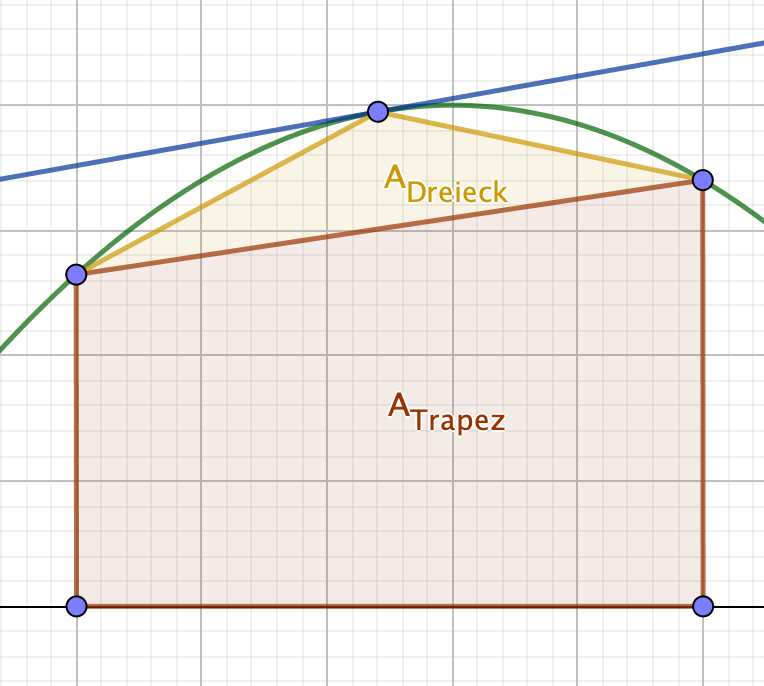
\includegraphics[width=5cm]{Kapitel_1/Grafiken/Grafik_1.png} \\
    $A_{Parabel} = A_{Trapez} + \frac{4}{3} A_{Dreieck}$
  \item Leibniz + Newton (~1670):
    $$ \int_a^b f(x) dx = F(b) - F(a),$$ wobei $\frac{d}{dx} F(x) = f(x)$
  \item Riemann (~1850): 
    $$ \int_a^b f(x) dx = \lim\limits_{\vert \Delta \vert \to \infty} \sum_{j=1}^n f(\xi_j)(x_j - x_{j-1}),$$
    wobei $\Delta = (x_0,...,x_n)$ Gitter Zerlegung von $[a, b]$, $a=x_0 < ...< x_n = b$, $\xi_j \in [x_{j-1}, x_j]$ und $\vert \Delta \vert := \max_{j=1,...n} \vert x_j - x_{j-1} \vert$.
    Das Riemannintegral existiert, falls: 
    $$ \forall \varepsilon > 0 \exists \delta > 0: \vert \Delta \vert < \delta \Rightarrow \vert \int_a^b f(X) dx - \sum_{j=1}^n f(\xi_j)(x_j-x_{j-1}) \vert < \varepsilon $$
\end{enumerate}
\end{example}

\begin{comment}[Approximation von Integralen]\leavevmode
\begin{enumerate}
  \item (linke) Rechtecksregel: 
    $$\int_{x_{j-1}}^{x_{j-1}+h} f(x) dx \approx h f(x_{j-1})$$
    $$\int_a^b f(x) dx = \sum_{j=1}^n \int_{x_{j-1}}^{x_j} f(x)dx \approx \sum_{j=1}^n f(x_{j-1}) (x_j-x_{j-1})$$
  \item Mittelpunktsregel:
    $$\int_{x_{j}}^{x_{j}+h} f(x) dx \approx f\left(\frac{x_j+x_j+h}{2}\right)h$$
    $$\int_a^bf(x)dx \approx \sum_{j=1}^n f\left( \frac{x_{j-1} + x_j}{2}\right) (x_j - x_{j-1})$$
    Da mit Hilfe der Transformationsformel sich jedes Integral $\int_{x_{j-1}}^{x_j}$ auf ein Integral $\int_a^b$ transformieren lässt, betrachten wir ohne Einschränkungen Integrale von $0$ bis $1$. Nutze dazu die Abb. $[a, b] \rightarrow [x_{j-1}, x_j], t \mapsto x_{j-1} + t(x_j - x_{j-1})$.
    $$ \int_{x_{j-1}}^{x_j} f(x) dx = \int_0^1 \underbrace{f\left( x_{j-1} + t(x_j - x_{j-1})\right)}_{:= g_{j-1}(t)} (x_j - x_{j-1})dt = \int_0^1 g_{j-1}(t)(x_j-x_{j-1})dt$$
\end{enumerate}
\end{comment}

\begin{definition}[Quadraturformel]
Eine s-stufige Quadraturformel zur Approximation von $\int_0^1 g(t)dt$ mit Knoten $c_i$ und Gewichten $b_i$ für $i=1,...s$ ist gegeben durch 
$$\sum_{i=1}^s b_i g(c_i) \left( \approx \int_0^1 g(t) dt\right)$$

\end{definition}

\begin{example}\leavevmode
\begin{enumerate}
  \item Rechtecksregel: $s = 1, b_1 = 1, c_1 = 0$
    $$ \int_0^1 g(t) \approx b_1 g(c_1) = g(0)$$
  \item Mittelpunktsregel: $s = 1, b_1 = 1, c_1 = \frac{1}{2}$
    $$ \int_0^1 g(t) \approx g(\frac{1}{2})$$
  \item Trapezregel: $s=2, b_1=b_2= \frac{1}{2}, c_1 = 0, c_2 = 1$
    $$ \int_0^1 g(t) \approx \frac{1}{2} g(0) + \frac{1}{2}g(1)$$
  \item Simpsonregel: $s=3, b_1 =  \frac{1}{6}, b_2 =  \frac{2}{3}, b_3 =  \frac{1}{6}, c_1 = 0, c_2 =  \frac{1}{2}, c_3 = 1$
    $$ \int_0^1 g(t) \approx \frac{1}{6} \left(g(0) + 4g\left(\frac{1}{2}\right) +g(1)\right)$$ 
    \textbf{Herleitung:} Man legt eine Parabel $p$ durch die Punkte $(0, g(0)), (\frac{1}{2}, g(\frac{1}{2})), (1, g(1))$ und integriert $p$ von 0 bis 1. \\
    $p(t) = g(0)(1-t)2(\frac{1}{2}-t) + g(\frac{1}{2})(1-t)4t + g(1)(\frac{1}{2}-t)2t$ \\
    $$\Rightarrow \int_0^1 p(t)dt = \frac{1}{6}g(0)+ \frac{2}{3}g(\frac{1}{2}) +\frac{1}{6}g(1)$$ 
  \item "pulcherrima et utilissima regula" von Newton:
    $$\int_0^1 g(t) dt \approx \frac{1}{8}\left(g(0) + 3g(\frac{1}{3}) + 3g(\frac{2}{3}) + g(1)\right)$$
\end{enumerate}

\end{example}

\begin{comment}[Monte-Carlo Integration]\leavevmode
\begin{enumerate}
  \item Eindimensionale Monte-Carlo Integration: \\
    Sei $a, b \in \mathbb{R}$, $a<b$. Wählt man $N$ unabhängige gleichverteilte Punkte $x_i$ in $[a,b]$ so gilt die Approximation:
    $$\int_a^b f(x) dx \approx \frac{1}{N} \sum_{j=1}^N (b-a)f(x_j)$$
    Nach dem Gesetz der großen Zahlen konvergiert dieser Ausdruck, falls 
    $$\int_a^b\vert f(x) \vert dx < \infty, \int_a^b f^2(x)dx < \infty$$
  \item Mehrdimensionale Monte-Carlo Integration: \\
    Sei $W=\otimes_{i=1}^d [a_i, b_i]$ ein d-dimensionaler Quader. Wählt man in W unabh. gleichvert. Zufallsvektoren $x_i$ in W, so ist
    $$\int_W f(x)dx \approx \frac{1}{N} Vol(W) \sum_{i=1}^N f(x_i),$$
    wobei $f:\mathbb{R}^d \rightarrow \mathbb{R}$.\\
    \textbf{Achtung:} Dieses gewöhnliche MC-Verfahren konvergiert sehr langsam. Verbesserungen sind z.B.: Importance sampling, Control variates, Antithetic variates und statified sampling.
\end{enumerate}
\end{comment} %Einführung
\subsection{Ordnung von Quadraturformeln}

\begin{definition}
Eine Quadraturformel (QF) mit Gewichten und Knoten $(b_i, c_i)_{i=1}^{s}$ hat \textbf{Ordnung p}, falls sie exakt ist für alle Polynome von Grad $ \leq p-1$.\\
$$\mathcal{P} := \left\{ \sum_{i=0}^{n}a_iX^i, a_i \in \mathbb{R} (\mathbb{C}) \right\}, \quad \text{Menge aller Polynome}  $$
Für $q \in \mathcal{P}$ ist $\text{deg}(q)$ der Grad des Polynoms.
\end{definition}

\begin{theorem}
Ein QF $(b_i, c_i)_{i=1}^{s}$ für $[0,1]$ hat Ordnung $p$ genau dann, wenn

$$\sum_{i=1}^{s} b_i c_i^{q-1} = \frac{1}{q}$$ für $q = 1,..,p$.
\begin{proof}[Beweis]
\begin{description}
  \item
\end{description}
\begin{description}
  \item $"\Rightarrow"$ \\
  QF hat Ordnung p $\Rightarrow$ QF ist exakt für $g(t) = t^{q-1}$ für $q = 1,..,p$ auf $[0,1]$ \\
  $\Rightarrow$ $$\sum b_i c_i^{q-1} = \int_{0}^{1} t^{q-1} dt = [\frac{t^q}{q}]_{t=0}^{1} = \frac{1}{q}$$
  \item $"\Leftarrow"$\\
  Jedes Polynom von Grad $p-1$ lässt sich als Linearkombination von $1, t, t^2, ...,t^{p-1}$. Die Behauptung folgt aus der Linearität in $g$ von $$\int_{0}^{1} g(t) dt$$ und $$\sum_{i=1}^{s}b_i g(c_i)$$
\end{description}
\end{proof}
\end{theorem}

\begin{example}
\begin{description}
  \item
\end{description}

\begin{enumerate}
  \item Rechtecksregel: $p=1$
  \item Mittelpunktsregel: $p=2$
  \item Trapezregel: $p=2$
  \item Simpsonregel: $p \geq 3$ nach Konstruktion \\
  \begin{align*}
  q &= 4: \quad \frac{1}{6} * 0^3 + \frac{4}{6} * \left(\frac{1}{2}\right)^3 + \frac{1}{6}*1^3 = \frac{1}{4} &\\
  q &= 5: \quad \frac{1}{6} * 0^4 + \frac{4}{6} * \left(\frac{1}{2}\right)^4 + \frac{1}{6}*1^4 = \frac{5}{24} \neq \frac{1}{5}&\\
  \end{align*}
  Nach Satz (2.2) ist damit die Ordnung der Simpsonregel $p=4$.
  \item "pulcherina et utilissima": Übung
\end{enumerate}
\end{example}

\begin{comment}
Zu vergebenen paarweise verschiedenen Knoten $c_1, ..., c_s$ lässt sich mit Satz (2.2) für $p=s$ ein lineares Gleichungssystem für die Gewichte $b_1, ..., b_s$ aufstellen.\\

$$
\underbrace{\left[ \begin{array}{rrrr}
1 & 1 & ... & 1 \\
c_1 & c_2 & ... & c_s \\
... & ... & ... & ... \\
c_1^{s-1} & c_2^{s-1} & ... & c_s^{s-1} \\
\end{array}\right]}_{= V}
*
\left[ \begin{array}{r}
b_1 \\
b_2 \\
... \\
b_s \\
\end{array}\right] 
= 
\left[ \begin{array}{r}
1 \\
1/2 \\
... \\
1/s \\
\end{array}\right] 
$$
Falls die Vandermonde-Matrix V invertierbar ist, so lassen sich die Gewichte $b_1, ..., b_s$ bestimmen, sodass die QF $(b_i, c_i)_{i = 1}^{s}$ mindestens Ordnung $s$ hat.
\end{comment}

\begin{definition}
Eine QF heißt symmetrisch, falls für $i = 1,...,s$ gilt:
\begin{enumerate}
  \item $c_i = 1 - c_{s+1-i}$
  \item $b_i = b_{s+1-i}$
\end{enumerate}
\end{definition}

\begin{example}[Symmetrische QF]
Mittelpunktsregel, Trapezregel, Simpsonregel,...
\end{example}

\begin{theorem}
Die maximal erreichbare Ordnung einer symmetrischen QF ist gerade.
\begin{proof}[Beweis]
Sei die QF $(b_i,c_i)_{i=1}^{s}$ exakt for Polynome vom Grad $\leq 2m-2$ (für $m \in \mathbb{N}$), (dann ist die Ordnung $\geq 2m-1$).
$$\forall g \in \mathcal{P}: deg(g) \leq 2m-2 \Rightarrow \sum_{i=1}^{s} b_i g(c_i) = \int_{0}^{1} g(t) dt$$
Sei $f \in \mathcal{P}$ mit $deg(f) = 2m-1$. \\
Wir zeigen QF ist exakt für $f$. 
$$f(t) = ct^{2m-1} + g(t)$$
für $g \in \mathcal{P}$ mit $deg(g) \leq 2m-2$ mit $c \neq 0$. \\
Trick: $f(t) = c(t-\frac{1}{2})^{2m-1} + \tilde{g}(t)$ mit $\tilde{g} \in \mathcal{P}$ und $deg(\tilde{g}) \leq 2m-2$

\begin{enumerate}
  \item Für $\tilde{g}$ ist die QF exakt
  \item $$\int_0^1 (t-\frac{1}{2})^{2m-1} dt = \left[\frac{1}{2m-2}(t-\frac{1}{2})^{2m-2}\right]_0^1 = 0$$
  $$ \sum_{i=1}^{s} b_i (c_i - \frac{1}{2})^{2m-1}$$ 
  Symmetrie $\Rightarrow$
  $$= \sum_{i=1}^{s} b_{s+1-i} (\frac{1}{2} - c_{s+1-i})^{2m-1} $$
  Definiere $j := s+1-i$
  $$ = \sum_{i=1}^{s} b_i \frac{1}{2} - c_i)^{2m-1} = -\sum_{i=1}^{s} b_i (c_i - \frac{1}{2})^{2m-1}$$
  $$\Rightarrow 2*\sum_{i=1}^{s} b_i (c_i - \frac{1}{2})^{2m-1} = 0$$
  $$\Rightarrow \sum_{i=1}^{s} b_i (c_i - \frac{1}{2})^{2m-1} = 0$$
  $$\sum_{i=1}^{s}b_if(c_i) = c \sum_{i=1}^{s}b_i(c_i-\frac{1}{2})^{2m-1} + \sum_{i=1}^{s}b_i\tilde{g}(c_i)$$
  $$ = c\int_0^1(t-\frac{1}{2})^{2m-1} dt + \int_0^1 \tilde{g}(t)dt = \int_0^1 f(t)dt$$
  $\Rightarrow$ QF hat mind. Ordnung $2m$.
\end{enumerate}
\end{proof}
\end{theorem}

\begin{theorem}
Sind Knoten $c_1 < c_2 < ... < c_s$ ($c_i \in \mathbb{R}, i = 1,...s$) gegeben, so existieren eindeutig bestimmte Gewichte $b_1 ,..., b_s$ derart, dass die QF $(b_i, c_i)_{i=1}^s$ die maximale Ordnung $p \geq s$ hat. \\
Es gilt $$b_i = \int_0^1 l_i(t) dt$$ mit $$l_i(t) = \frac{\prod_{j=1, j\neq i}^s (t-c_j)}{\prod_{j=1, j\neq i}^s (c_i-c_j)}$$

\begin{proof}[Beweis] von 2.8 \\
\begin{enumerate}
  \item Hat die QF die Ordnung $p \geq s$, so ist wegen $deg(l_i) = s-1)$:
  $$ \int_0^1 l_i(t) dt = \sum_{j=1}^s b_j l_i(c_j) = b_i$$
  \item Zu den Knoten $c_i, ...c_s$ definiere $b_i$ wie angegeben. Die QF ist dann exakt für alle Polynome von Grad $ \leq s-1$, da die $l_1, ...,l_s$ linear unabhängig sind und eine Basis des Vektorraums der Polynome von Grad $\leq s-1$ bilden.
\end{enumerate}
\end{proof}
\end{theorem}

\begin{comment*}[zu Satz (2.8)]
$l_i$ ist das i-te Lagrangepolynom zu den Knoten $c_1, ...,c_s$. Es gilt:
\begin{enumerate}
  \item $deg(l_i) = s-1$
  \item $l_i(c_j) = \left\{
\begin{array}{ll}
0 & \,i \neq j \\
1 & \, i = j\\
\end{array}
\right. $, für $j=1,...,s$
\end{enumerate}

\end{comment*}
 %Ordnung von Quadraturformeln
\subsection{Quadraturfehler}

Allgemeine Voraussetzung $f:[a,b] \rightarrow \mathbb{R}$ sei hinreichend oft differenzierbar ($f$ ist eine glatte Funktion)

\begin{definition}
Der Fehler bei der Approximation des Integrals durch die QF ist 
$$ err = \int_a^b f(x)dx = \sum_{j=0}^{n-1} h_{j+1} \sum_{i=1}^s b_i f(x_j+h_{j+1}c_i)$$
mit $h_{j+1} = x_{j+1}-x_j$
$$ = \sum_{j=0}^{n-1} \int_{x_j}^{x_{j+1}} f(x_j + \tau) d\tau - h_{j+1} \sum_{i=1}^s b_i f(x_j + h_{j+1}c_i)$$
$$ = \sum_{j=0}^{n-1} h_{j+1} \int_0^1 g_j(\xi) d\xi -h_{j+1} \sum_{i=1}^s b_i g_j(c_i)$$
mit $ g_j(\xi) = f(x_j + \xi h_{j+1})$. \\
Der Quadraturfehler auf Teilintervallen $[x_j, x_j+h_{j+1}]$ ist 
$$E(f, x_j, h_{j+1}) = \int_{x_j}^{x_{j+1}} f(x)dx  - h_{j+1} \sum_{i=1}^s b_i f(x_j + c_i h_{j+1})$$
$$= h_{j+1} \left( \int_0^1 g_j(\xi) d\xi - \sum_{i=1}^s b_i g_j(c_i) \right)$$ 
\end{definition}

\begin{nothing}[Fehlerabschätzung - 1. Versuch]
Falls $f$ auf $[x_0, x_0+h]$ glatt genug ist und die QF Ordnung $p$ hat, aber nicht Ordnung $p+1$, so erhält man durch Taylorentwicklung um $x_0$ von $f(x_0 + \xi h) = g_0(\xi)$ und $f(x_0+c_ih)$:
$$E(f, x_0, h) = \sum_{k\geq 0} \frac{h^{k+1}}{k!} \left( \int_0^1 t^k dt - \sum_{i=1}^s b_i c_i^k \right) f^{(k)}(x_0)$$
$$= \frac{h^{p+1}}{p!} \left( \frac{1}{p+1} - \sum_{i=1}^s b_i c_i^p\right) f^{(p)}(x_0) + \underbrace{\mathcal{O}(h^{p+2})}_{Taylerrestglied}$$
Die Konstante $C = \frac{1}{p!} \left( \frac{1}{p+1} - \sum_{i=1}^s b_i c_i^p \right)$ heißt Fehlerkonstante. \\
Ist $h$ klein genug, sodass das Taylorrestglied im Vergleich zu $h^{p+1}C f^{(p)}(x_0)$ vernachlässigbar ist, so gilt:
$$ err = \sum_{j=0}^{n-1} E(f, x_j, h), $$ 
mit $ x_j = x_0+jh$
$$ \approx Ch^p \sum_{j=0}^{n-1} hf^{(p)}(x_j)$$ 
$$\approx Ch^p \int_a^b f^{(p)}(x)dx$$ 
$$= Ch^p \left(f^{(p-1)}(b) - f^{(p-1)}(a) \right)$$
\end{nothing}

\begin{nothing}[Rigorose Fehlerabschätzung]
\begin{description}
  \item
\end{description}
\begin{description}
  \item \textbf{Satz 1:} \\
    Sei $f: [a, b] \rightarrow \mathbb{R}$ $k$-mal stetig differenzierbar ($f \in C^k([a, b])$) und habe die QF Ordnung $p$, so gilt für $h < b-a$ und $k \leq p$\\
    $$E(f, x_0, h) = h^{k+1} \int_0^1 K_k(\tau) f^{(k)}(x_0+\tau k) d\tau,$$
    wobei der Peanokern $K_k(\tau)$ durch 
    $$ K_k(\tau) := \frac{(1-\tau)^k}{k!} - \sum_{i=1}^s b_i \frac{(c_i - \tau)^{k-1}_+}{(k-1)!}, $$
    mit 
    $(\sigma)_+^{k-1} = \left\{
    \begin{array}{ll}
    \sigma ^{k-1} &  \sigma > 0 \\
    0 & \, \textrm{sonst} \\
    \end{array}
    \right. $, gegeben ist.
  \item \begin{proof}[Beweis] 
    Taylorentwicklung mit Integralrestglied und Transformation 
    $$f(x_0 + th) = \sum_{j=0}^{k-1} \frac{(th)^j}{j!} f^{(j)}(x_0) + h^k \int_0^t \frac{(t-\tau)^{k-1}}{(k-1)!} f^{(k)}(x_0+\tau h) d\tau$$
    eingesetzt in (*) und die Verwendung von 
    $$\int_0^{c_i} (c_i - \tau)^{k-1} g(\tau) d\tau = \int_0^1 (c_i-\tau)_+^{k-1} g(\tau) d\tau$$
    liefern
    \begin{multline*} 
    E(f, x_0, h)= h 
      \int_0^1 
        \left( 
          \sum_{j=0}^{k-1} 
            \frac{(th)^j}{j!} f^{(j)}(x_0) + h^k 
            \int_0^t 
              \frac{(t-\tau)^{k-1}}{(k-1)!} f^{(k)}(x_0+\tau h) 
            d\tau 
        \right)
      dt - \\h
      \sum_{i=1}^s b_i 
        \left( 
          \sum_{j=0}^{k-1} 
            \frac{(c_ih)^j}{j!} f^{(j)}(x_0) + h^k 
            \int_0^{c_i} 
              \frac{(c_i-\tau)^{k-1}}{(k-1)!} 
              f^{(k)}(x_0+c_ih) 
            d\tau
        \right)
    \end{multline*}
    
    \begin{displaymath}
    \underbrace{=}_{k\leq p} h h^k \left[ \int_0^1 \int_0^t \frac{(t-\tau)^{k-1}}{(k-1)!} f^{(k)} (x_0 + \tau h) d\tau dt - \sum_{i=1}^s \int_0^1 \frac{(c_i-\tau)^{k-1}_+}{(k-1)!} f^{(k)}(x_0+\tau h) d\tau \right]
    \end{displaymath}
    
    \begin{displaymath}
    = h h^k \left[ \int_0^1 \int_0^1 \frac{(t-\tau)^{k-1}_+}{(k-1)!} f^{(k)}(x_0+\tau h) d\tau dt - \sum_{i=1}^s b_i \int_0^1 \frac{(c_i - \tau)^{k-1}_+}{(k-1)!} f^{(k)}(x_0+\tau h) d\tau \right] 
    \end{displaymath}
    
    \begin{displaymath}
    = h^{k+1} \int_0^1 \left( \int_0^1 \frac{(t-\tau)_+^{k-1}}{(k-1)!} dt - \frac{(c_i - \tau)_+^{k-1}}{(k-1)!} \right) f^{(k)}(x_0+\tau h) d\tau
    \end{displaymath}
    
    \begin{displaymath}
    = h^{k+1} \int_0^1 K_k(\tau) f^{(k)}(x_0+\tau h) d\tau
    \end{displaymath}
    
    , da
    \begin{displaymath}
    \int_0^1 \frac{(t-\tau)^{k-1}_+}{(k-1)!} dt
    = \int_0^1 \frac{(t-\tau)^{k-1}}{(k-1)!}
    = \left[ \frac{1}{k!} (t-\tau)^k \right]_{t=\tau}^1
    = \frac{1}{k!} (1-\tau)^k
    \end{displaymath}
    \end{proof}
    
  \item \textbf{Satz 2:} (Eigenschaften des Peanokerns) \\
    Für eine QF der Ordnung $p$ gilt für $k \leq p$ ($k, p \in \mathbb{N}$) 
    \begin{enumerate}
      \item $K_k'(\tau) = -K_{k-1}(\tau)$ für $k \geq 2$ und $\tau \neq c_i$ falls $k=2$
      \item $K_k(1) = 0$ für $k \geq 1$, falls $c_i \leq 1$ für $i=1,..., s$
      \item $K_k(0) = 0$ für $k \geq 2$, falls $c_i \leq 1$ für $i=1,..., s$
      \item $\int_0^1 K_p(\tau) = \frac{1}{p!} \left(\frac{1}{p-1} - \sum_{i=1}^s b_i c_i^p \right)=: C$ (Fehlerkonstante $C$ aus (3.2))
      \item $K_1(\tau)$ ist stückweise linear mit Steigung $-1$ und Sprüngen der Höhe $b_i$ an den Stellen $c_i$
    \end{enumerate}
  
  \item
  \begin{proof}[Beweis]
    Eventuell Übungsaufgabe
  \end{proof}
  
  \item \textbf{Beispiel:} \\
    Mittelpunktsregel: 
      $$K_1(\tau) = \frac{(1-\tau)^1}{1!} - 1 \frac{(\frac{1}{2} - \tau)^1_+}{0!}$$
      $$= 1- \tau - \left( \frac{1}{2} - \tau \right)_+^0$$
      $$ = \left\{
        \begin{array}{ll}
        1-\tau - 1  & \tau < \frac{1}{2} \\
        1-\tau & \, \tau \geq \frac{1}{2} \\
        \end{array}
      \right. $$
      
      $$K_2(\tau) = \frac{(1-\tau)^2}{2!} - 1 \frac{(\frac{1}{2} - \tau)^1_+}{1!}$$
      $$= \frac{1}{2} (1-\tau)^2 - \left( \frac{1}{2} - \tau \right)_+^1$$
      $$ = \left\{
        \begin{array}{ll}
        \frac{\tau^2}{2}  & \tau < \frac{1}{2} \\
        \frac{1}{2}(1-\tau)^2 & \, \tau \geq \frac{1}{2} \\
        \end{array}
      \right. $$
    
    \item \textbf{Satz 3:} \\
      Sei $f \in C^k([a,b])$ und habe die QF $(b_i, c_i)^s_{i=1}$, Ordnung $p \geq k$, so gilt für den Fehler $err$ aus $(3.1)$ 
      $$ \vert err \vert \leq h^k (b-a) \int_0^1 \vert K_k(\tau) \vert d\tau \max_{x \in [a,b]} \vert f^{(k)}(x) \vert$$
      mit $h = \max_{j=1,..,n} h_j$
    
    \item \begin{proof}[Beweis]
      Mit Satz $1$ gilt 
      $$ \vert E(f, x_j, h_{j+1}) \vert \leq h_{j+1}^{k+1} \int_0^1 \vert K_k(\tau) \vert \vert f^{(k)}(x_j+\tau h_{j+1}) \vert d\tau$$
      $$ \leq h_{j+1}^{k+1} \int_0^1 \vert K_k(\tau) \vert d\tau \max_{x \in [x_j, x_j + h_{j+1}]} \vert f^{(k)}(x) \vert $$
      Für 
      $$ \vert err \vert = \vert \sum_{j=0}^{n-1} E(f, x_j, h_{j+1}) \vert $$
      $$ \leq \sum_{j=0}^{n-1} \vert E(f, x_j, h_{j+1}) \vert $$
      $$ \leq \underbrace{\sum_{j=0}^{n-1} h_{j+1}}_{b-a} \underbrace{h_{j+1}^k}_{\leq h^k} \int_0^1 \vert K_k(\tau) \vert d\tau \underbrace{\max_{x \in [x_j, x_{j+1}]} \vert f^{(k)} (x) \vert}_{\leq \max_{x\in[a,b] \vert f^{(k)}(x) \vert}}$$
    \end{proof}
    
    \item \textbf{Beispiele} \\
      Für die Mittelpunktsregel (maximale Ordnung = 2) erhält man
      $$ \vert err \vert \leq h^2 (b-a) \frac{1}{24} \max_{x\in[a,b]} \vert f^{(2)}(x) \vert $$ 
      Für die Trapezregel (maximale Ordnung = 2)
      $$ \vert err \vert \leq h^2 (b-a) \frac{1}{12} \max_{x\in[a,b]} \vert f^{(2)}(x) \vert $$  
      Für die Simpsonregel (maximale Ordnung = 4)
      $$ \vert err \vert \leq h^4 (b-a) \frac{1}{2880} \max_{x\in[a,b]} \vert f^{(4)}(x) \vert $$ 
      $\rightarrow$ Der Fehler wird klein, falls $h$ klein und die Ordnung $p$ groß wird.
\end{description}
\end{nothing} %Quadraturfehler
\subsection{Quadratur mit hoher Ordnung}
$c_1< ... < c_s$ Knoten gegeben. Aus $\S2$ wissen wir: \\
Es gibt Gewichte $b_1, ..., b_s$, sodass $p \leq s$. \\
\underline{Fragen:} 
\begin{itemize}
  \item Kann man $c_j$ so wählen, dass $p>s$?
  \item Wenn ja, wie?
  \item Wie groß kann $p$ maximal werden?
\end{itemize}
\underline{Ziel:} QF mit Ordnung $p=s+m$ für $m \in \mathbb{N}, m > 1$
Sei $g \in \mathcal{P}_{s+m-1}$ (Polynome von Grad $\leq s+m-1$).\\
$g$ soll durch die QF exakt integriert werden.\\
\underline{Idee:} Dividiere $g$ durch $M(t) = \prod_{i=1}^s (t-c_i)$ "Knotenpolynom"\\
$deg(M) = s$ \\
$g(t) = M(t) h(t) + r(t)$ mit Rest $r$, $deg(r) \leq s-1$ und $deg(h) \leq m-1$ \\
Dann gilt einerseits
$$\int_0^1 g(t)dt = \int_0^1 M(t)h(t)dt + \int_0^1r(t)dt$$
und andererseits
\begin{gather*}\sum_{i=1}^s b_ig(c_i) = \sum_{i=1}^s b_i \underbrace{M(c_i)}_{= 0} h(c_i) + \sum_{i=1}^s b_ir(c_i) \\
 = 0 + \int_0^1 r(t)dt,\end{gather*}
 da $p \leq s$\\
Damit ist gezeigt:

\begin{theorem}
Sei $(b_i, c_i)_{i=1}^s$ der Ordnung $p \geq s$. Äquivalent sind:
\begin{enumerate}
  \item QF hat Ordnung $s+m$
  \item $\forall h \in \mathcal(P)_{m-1}:\int_0^1 M(t)h(t)dt = 0$
\end{enumerate}
\end{theorem}

\begin{korollar}
Die Ordnung einer $s$-stufigen QF ist höchstens $2s$
\begin{proof}[Beweis (indirekt)]
Annahme: $p > 2s$ \\
$$(4.1) \Rightarrow \forall h \in \mathcal{P}_s: \int_0^1 M(t)h(t)dt = 0 $$
Setze $h=M$, dann ist $$ \int_0^1 M(t)^2dt = 0$$
$\lightning$ zu $\int_0^1 M(t)^2 dt > 0$, da $M(t) \equiv 0$
\end{proof}
\end{korollar}

\begin{nothing}[Beispiele/Korollare]
\begin{description} \item \end{description}
\begin{enumerate}
  \item Jede 3-stufige QF mit Ordnung $\geq 4$ muss
    $$\int_0^1 (t-c_1)(t-c_2)(t-c_3)dt = 0$$
    $$\int_0^1 t^3 + t^2(-c_1-c_2-c_3) + t(c_1c_2+c_2c_3+c_1c_3) - c_1c_2c_3 dt$$
    $$ = \frac{1}{4} + \frac{1}{3}(-c_1-c_2-c_3) + \frac{1}{2}(c_1c_2 + c_2c_3 + c_1c_3) - c_1c_2c_3$$
    erfüllen, dh
    $$ c_3 = \frac{\frac{1}{4} - (c_1+c_2)\frac{1}{3} + c_1c_2 \frac{1}{2}}{\frac{1}{3} - (c_2+c_1)\frac{1}{2} + c_1c_2}$$
    
  \item Zur Berechnung der Knoten einer $3$-stufigen QF der Ordnung $6$ verwenden wir $(4.2)$ mit $h(t) = 1, t, t^2$
    $$\int_0^1 M(t)h(t) = 0$$
    \begin{description}
      \item $h(t) = 1 \rightarrow c_1c_2c_3 - \frac{1}{2}(c_1c_2 + c_2c_3 + c_1c_3) + \frac{1}{3}(c_1+c_2+c_3) = \frac{1}{4}$
      
      \item $h(t) = t \rightarrow \frac{1}{2}c_1c_2c_3 - \frac{1}{3}(c_1c_2 + c_2c_3 + c_1c_3) + \frac{1}{4}(c_1+c_2+c_3) = \frac{1}{5}$
      
      \item $h(t) = t^2 \rightarrow \frac{1}{3}c_1c_2c_3 - \frac{1}{4}(c_1c_2 + c_2c_3 + c_1c_3) + \frac{1}{5}(c_1+c_2+c_3) = \frac{1}{6}$
    \end{description}
    nichtlineares Gleichungssystem in $c_1, c_2, c_3$ \\
    \underline{Trick:}
    \begin{description}
      \item $\sigma_1 = c_1+c_2+c_3$
      \item $\sigma_2 = c_1c_2 + c_1c_3 + c_2c_3$
      \item $\sigma_2 = c_1c_2c_3$
    \end{description} 
    Das sind die Koeffizienten von $M(t)$ in der Monombasis. \\
    $M(t) = (t-c_1)(t-c_2)(t-c_3) = t^3 - \sigma_1t^2 + \sigma_2t - \sigma_3$ \\
    und das Gleichungssystem ist linear in $\sigma_1, \sigma_2, \sigma_3$ \\
    mit Lösung $\sigma_1 = \frac{3}{2}, \sigma_2 = \frac{3}{5}, \sigma_3 = \frac{1}{20}$ \\
    und damit ist $M(t) = t^3 - \frac{3}{2}t^2 + \frac{3}{5}t - \frac{1}{20}$ \\
    $ = (t-\frac{1}{2})(t-\frac{5-\sqrt{15}}{10})(t-\frac{5 + \sqrt{15}}{10})$ \\
    Glücklicherweise sind die Wurzeln von $M(t)$ in $[0,1]$. Damit lassen sich die Gewichte mit $(2.4)$ berechnen und wir erhalten
    $$\int_0^1 g(t) dt = \frac{5}{18} g\left(\frac{5-\sqrt{15}}{10}\right) + \frac{8}{18} g\left(\frac{1}{2}\right) + \frac{5}{18}g\left(\frac{5+\sqrt{15}}{10}\right)$$
    \underline{Ziel:} Konstruktion von QF der Ordnung $2s$ mit Hilfe von orthogonalen Polynomen.
\end{enumerate}
\end{nothing}
 %Quadratur mit hoher Ordnung
\subsection{Orthogonalpolynome}
Bedingung $2.$ in Satz $(4.1)$ 
$$ \forall h \in \mathcal{P}_{m-1}: \int_0^1 M(t)h(t) = 0$$
kann als Orthogonalitätsbedingung bzgl. eines Skalarprodukts $\langle f, g\rangle = \int_0^1 f(t)g(t)dt$ auf dem Vektorraum $L^2([0,1])$ oder $C([0,1])$ aufgefasst werden. \\
\underline{Erinnerung:}
$$\mathcal{P}_s := \left\{ \sum_{j=0}^s \alpha_j X^j, \alpha_j \in \mathbb{R} \right\}$$ 
ist ein $\mathbb{R}$-VR mit $dim(\mathcal{P}_s) = s+1$ und Basis $\left\{ 1, X, X^2, ..., X^s \right\}$\\ \\
$\langle\cdot,\cdot\rangle : C([0,1]) \times C([0,1]) \rightarrow \mathbb{R}, (f, g) \mapsto \int_0^1 f(t)g(t)dt$ ist 
\begin{enumerate}
  \item symmetrisch $ \langle f, g\rangle = \langle g, f\rangle$
  \item linear $\langle \alpha f + g, h\rangle = \alpha \langle f, h\rangle + \langle g, h\rangle$
  \item positiv definit $\langle f, f\rangle \geq 0 $ und $ \langle f, f\rangle = 0 \Rightarrow f = 0$
\end{enumerate}
Wie in der linearen Algebra definieren wir $f$ steht senkrecht auf $g$: $f \perp g \Leftrightarrow \langle f, g\rangle = 0$

\begin{theorem}
QF hat die Ordnung $s+m \Leftrightarrow $ M ist orthogonal auf allen Polynome in $\mathcal{P}_{m-1}$
\end{theorem}

\begin{definition}
Für eine Gewichtsfunktion $\omega : (a, b) \rightarrow \mathbb{R}$ mit 
\begin{enumerate}
  \item $\omega$ stetig
  \item $\forall x\in(a,b): \omega(x) > 0 $
  \item $\forall k \in \mathbb{N}: \int_a^b \omega(x) \vert x \vert^k dx < \infty$
\end{enumerate}
definieren wir auf den Vektorraum 
$$ V = \left\{ f: [a,b] \rightarrow \mathbb{R}: f \medspace stetig \medspace und \int_a^b f(x)^2 \omega(x) dx < \infty \right\} $$
das gewichtete Skalarprodukt
$$ \langle f, g \rangle_\omega := \int_a^b \omega(x)f(x)g(x)dx$$
für $f, g \in V$ \\
$f \perp_\omega g :\Leftrightarrow \langle f, g, \rangle_\omega = 0$
\end{definition}

\begin{theorem}
Es existiert eine eindeutige Folge von Polynomen $p_0, p_1, ...$ mit 
\begin{enumerate}
  \item $deg(p_k) = k$
  \item $\forall q \in \mathcal{P}_{k-1}:p_k \perp q$ für $k \geq 1$
  \item $p_k(x) = x^k + r$ mit $deg(r) \leq  k-1$ "Normierung"
\end{enumerate}
Diese Polynome lassen sich rekursiv berechnen durch \\
$ p_{k+1}(x) := (x- \beta_{k+1}) p_k(x) - \gamma_{k+1}^2 p_{k-1}(x)$ für $k \geq 1$ \\
$ p_0(x) := 1$, $p_{-1}(x) := 0$ \\
$ \beta_{k+1} := \frac{\langle xp_k, p_k \rangle}{\langle p_k, p_k \rangle}$ \\
$ \gamma_{k+1}^2 := \frac{\langle p_k, p_k \rangle}{\langle p_{k-1}, p_{k-1} \rangle}$
\begin{proof}[Beweis]
(vgl. Gram-Schmidt Orthogonalisierung LinA) \\
Sei $p_0, ..., p_k$ bereits bekannt. Zur Konstruktion von $p_{k+1}$ setzen wir
$$p_{k+1}(x) = xp_k(x) + \sum_{j=0}^{k} \alpha_j p_j(x)$$
(damit ist 3. erfüllt) \\
Zur Bestimmung der $\alpha_j$:
\begin{enumerate}
  \item $ 0 = \langle p_{k+1}, p_k \rangle = \langle xp_k, p_k \rangle + \alpha_k \langle p_k, p_k \rangle + \sum_{j=0}^{k-1} \alpha_j \underbrace{\langle p_j, p_k \rangle}_{= 0}$\\
    $\Rightarrow \alpha_k = -\frac{\langle xp_k, p_k \rangle}{\langle p_k, p_k \rangle} =: -\beta_{k+1}$
  
  \item $$0 = \langle p_{k+1}, p_{k-1} \rangle = \langle xp_k, p_{k-1} \rangle + 0 + \alpha_{k-1} \langle p_{k-1}, p_{k-1} \rangle + 0$$ 
    $$= \langle p_{k}, xp_{k-1} \rangle + \alpha_{k-1} \langle p_{k-1}, p_{k-1} \rangle$$ 
    Aufgrund von 3. $\Rightarrow$ 
    $$xp_{k-1} = p_k + r$$ mit $deg(r) \leq k-1$
    $$\Rightarrow \langle p_{k}, xp_{k-1} \rangle = \langle p_{k}, p_{k} \rangle + \underbrace{\langle p_{k}, r \rangle}_{= 0}$$ 
    $$\Rightarrow \alpha_{k-1} = - \frac{\langle p_k, p_k \rangle}{\langle p_{k-1}, p_{k-1} \rangle} =: -\gamma_{k+1}^2$$
  
  \item Für $j \leq k-2$:
    $$ 0 = \langle p_{k+1}, p_{j} \rangle = \langle xp_{k}, p_{j} \rangle + \alpha_j \langle p_{j}, p_{j} \rangle$$
    $$ = \underbrace{\langle p_{k}, xp_{j} \rangle}_{= 0} + \alpha_j \underbrace{\langle p_{j}, p_{j} \rangle}_{\neq 0}$$
    $\langle p_{k}, xp_{j} \rangle = 0$ gilt, da $deg(xp_j) \leq k+1$ \\
    Insgesamt haben wir
    $$p_{k+1}(x) = xp_k(x) - \beta_{k+1}p_k(x) - \gamma_{k+1}^2 p_{k-1}(x)$$
\end{enumerate}
\end{proof}
\end{theorem}

Für eine QF maximaler Ordnung müssen nach Satz (4.1) die Knoten $c_i$, $i=1, ...,s$ so gewählt werden, dass 
$$M(t) = \prod_{i=1}^s(t-c_i)$$
das Orthogonalpolynom vom Grad $s$ bezüglich des Skalarprodukts mit $\omega(x) \equiv 1$ auf $[0,1]$ ist. \\
\underline{Frage:} Sind die Wurzeln der Orthogonalpolynome aus (5.3) reell? (Spoiler: Ja)

\begin{theorem}
Sei $p_k$ das Orthogonalpolynom wie in (5.3) definiert (bzgl. $\langle f, g \rangle = \int_a^b f(x)g(x)\omega(x)dx$). Alle Wurzeln von $p_k$ sind einfach und liegen im offenen Intervall $(a,b)$.

\begin{proof}[Beweis]
Seie $x_1, ..., x_r$ jene Wurzeln in $p_k$, die reell sind, in $(a, b)$ liegen und bei denen $p_k$ das Vorzeichen wechselt (Wurzeln mit ungerader Vielfachheit). \\
Klar ist: $r \leq k$. \\
Sei 
$$g(x) = \prod_{j=1}^r (x-x_j)$$ 
Dann ist 
$$ \langle p_k, g \rangle = \int_a^b \underbrace{p_k(x) \thinspace g(x)}_{\text{Wechselt das Vorzeichen in (a,b) nicht}} \thinspace \omega(x) \thinspace dx \neq 0$$
Andererseits ist $p_k$ orthogonal zu allen Polynomen vom Grad $\leq k-1$ \\
$\Rightarrow r = deg(g) \geq k$ \\
$\Rightarrow r=k$
\end{proof}
\end{theorem}

\begin{example}[Orthogonale Polynome]
\begin{tabular}{llll}
 
Bezeichnung & (a,b) & w(x) & Name\\
 
& & & \\

$P_k$ & $(-1,1)$ & $1$ & Legendrepolynome \\

$T_k$ & $(-1,1)$ & $(1-x^2)^{-1/2}$ & Tschebyscheff-Polynome \\

$P_k^{(\alpha, \beta)}$ & $(-1,1)$ & $(1-x)^{\alpha}(1-x)^{\beta}$ & Jacobi-Polynome $\alpha, \beta > -1$ \\

$L_k^{(\alpha)}$ & $(0, \infty)$ & $x^{\alpha} e^{-x}$ & Laguere-Polynome \\

$M_k$ & $(-\infty,\infty)$ & $e^{-x^2}$ & Harmitepolynome \\

\end{tabular}\\
\underline{Bemerkung:} Teilweise sind andere Normierungen üblich $P_k(1) = 1$, $T_k(x) = 2^{k-1} x^k + ...$, ...
\end{example} %Orthogonalpolynome
\subsection{Ein adaptives Programm}

Gegeben sei eine QF mit $(b_i, c_i)_{i=1}^s$ mit Ordnung $p=2s$ (die höchste Ordnung, die es gibt) z.B. $s=15$ \\
\underline{Ziel:} Ein Computerprogramm adagaussqf(f, a, b, Tol), welches für eine Funktion $f$ auf dem Interval $[a, b]$ eine Approximation an $\int_a^b f(x) dx$ berechnet, sodass der Fehler $\leq$ Tol ist (für viele Funktionen). \\
Konstruiere eine Zerlegung $\Delta = \left\{ a = x_0 < ... < x_n = b\right\}$ des Intervalls, sodass für die Approximation 
$$I_\Delta := \sum_{j=0}^{n-1} h_{j+1} \sum_{i=1}^s b_if(x_i + c_ih_{j+1})$$
gilt 
$$\vert I_\Delta - \int_a^b f(x) dx \vert \leq Tol \int_a^b \vert f(x) \vert dx $$
Schwierigkeiten:

\begin{enumerate}
  \item[a)] Schätzung des Fehlers
  \item[b)] Wahl der Zerlegung des Intervalls 
\end{enumerate}

\begin{nothing}[Zerlegung des Intervalls]
Für ein Teilintervall $[x_j, x_{j+1}]$ von $[a,b]$ lassen sich 
$$res[x_j, x_{j+1}] := h_{j+1} \sum_{i=1}^s b_i f(x_j + c_i h_{j+1})$$
und
$$ resabs[x_j, x_{j+1}] := h_{j+1} \sum_{i=1}^s \vert b_i f(x_j + c_i h_{j+1}) \vert$$
berechnen.\\
Angenommen wir können eine Schätzung des Fehlers $err[x_, x_{j+1}]$ berechnen mit
$$err[x_, x_{j+1}] \approx res[x_, x_{j+1}] - \int_{x_j}^{x_{j+1}} f(x) dx,$$
dann bietet sich folgendes Verfahren zur Konstruktion einer Zerlegung an:
\begin{enumerate}
  \item Berechne $res[a,b]$, $resabs[a,b]$ und $err[a, b]$. \\
    Falls 
    $$\vert err[a,b] \vert \leq Tol \thinspace resabs[a,b]$$
    Gebe $res[a,b]$ zurück.\\
    Ansonsten:
    
  \item Zerlege $[a,b]$ in 
    $$I_0 = \left[a,\frac{b-a}{2}\right]$$
    und
    $$I_1 = \left[ \frac{b-a}{2}, b \right]$$
    und berechne 
    \begin{description}
      \item $res \thinspace I_0$, $resabs \thinspace I_0$, $err \thinspace I_0$ und
      \item $res \thinspace I_1$, $resabs \thinspace I_1$, $err \thinspace I_1$ 
    \end{description}
    n = 2.
    
  \item Falls 
    $$ \sum_{j=0}^{n-1} \vert err \thinspace I_j \vert \leq Tol \thinspace \sum_{j=0}^{n-1} resabs \thinspace I_j$$
    Gebe
    $$ \sum_{j=0}^{n-1} res \thinspace I_j$$
    zurück. Ansonsten: \\
    Unterteile das Intervall $I_k = [a_k, b_k]$, in dem der Fehler maximal ist in zwei Teilintervalle 
    $$I_l = \left[a_k,\frac{b_k-a_k}{2}\right]$$
    und
    $$I_m = \left[ \frac{b_k-a_k}{2}, b_k \right]$$
    und berechne:
    \begin{description}
      \item $res \thinspace I_l$, $resabs \thinspace I_l$, $err \thinspace I_l$ und
      \item $res \thinspace I_m$, $resabs \thinspace I_m$, $err \thinspace I_m$
    \end{description}
    $n =n+1$ \\
    Gehe zu 3)
\end{enumerate}
\end{nothing}

\begin{nothing}[Schätzung des Fehlers]
\underline{Ziel:} Berechne Approximation an 
$$\int_{x_j}^{x_{j+1}} f(x)dx - h_{j+1} \sum_{i=1}^s b_i f(x_j + h_{j+1} c_i)$$
ohne zusätzliche Funktionsauswertungen.\\
\underline{Idee:} Konstruiere eingebettete QF, d.h. QF zu den selben Knoten $c_i$ mit Gewichten $\hat{b}_i$ und Ordnung $\hat{p} < p$. \\
\underline{Bemerkung:} Falls $p=2s$ ist, so gilt $\hat{p} \leq s-1$ (wäre $\hat{p} \geq s$, so wäre nach (2.8) $\hat{b}_i = b_i$).\\
Eine Approximation des Fehlers für die eingebettete QF ist durch 
\begin{align*}
\text{diff} \thinspace [x_j, x_{j+1}] &= h_{j+1} \sum_{i=1}^s b_i f(x_j + c_i h_{j+1}) - h_{j+1} \sum_{i=1}^s \hat{b}_i f(x_j + c_i h_{j+1})&\\
&= h_{j+1} \sum_{i=1}^s (b_i - \hat{b}_i) f(x_j+c_i h_{j+1})
\end{align*}
gegeben. Es gilt
\begin{align*}
\text{diff} \thinspace [x_j, x_{j+1}] &= h_{j+1} \sum_{i=1}^s b_i f(x_j + c_i h_{j+1}) - \int_{x_j}^{x_{j+1}} f(x)dx &\\
& \quad - \left( h_{j+1} \sum_{i=1}^s \hat{b}_i f(x_j + c_i h_{j+1}) - \int_{x_j}^{x_{j+1}} f(x)dx \right)&\\
&= \text{Fehler der QF } (b_i, c_i)_{i=1}^s - \text{Fehler der QF } (\hat{b}_i, c_i)_{i=1}^s &\\
&= C_1 h_{j+1}^{p+1} + C_2h_{j+1}^{\hat{p}+1}
\end{align*}
Falls $h_{j+1}$ klein ist, ist $C_1 h_{j+1}^{p+1} << C_2h_{j+1}^{\hat{p}+1}$.\\
Drei Möglichkeiten den Fehler zu schätzen:
\begin{enumerate}
  \item[I)] $\text{err }[x_j, x_{j+1}] \approx \text{diff }[x_j, x_{j+1}]$. Sehr pessimistisch
  \item[II)] $\text{err }[x_j, x_{j+1}] \approx (\text{diff }[x_j, x_{j+1}])^2$, falls $p=2s$ und $\hat{p} = s-1$. Wenig verlässlich
  \item[III)] Verwende dritte eingebettete QF 
    \begin{description}
      \item $(\hat{\hat{b}}_i, c_i)$ der Ordnung 6 
      \item zu $(b_i, c_i)$ der Ordnung $30 = 2s$, $s=15$
      \item und $(\hat{b}_i, c_i)$ der Ordnung 14
      \item $\hat{\text{diff}} = h_{j+1} \sum_{i=1}^s (b_i - \hat{\hat{b}}_i) f(x_{j} + c_i h_{j+1}) \approx C_3 h^7$
      \item 
        \begin{align*}
        \text{err }[x_j, x_{j+1}] &= \text{diff }[x_j, x_{j+1}] \left( \frac{\text{diff}}{\hat{\text{diff}}} \right) ^2&\\
        &= C_2 \frac{C_2^2}{C_3^2} h_{j+1}^{15} \left( \frac{h_{j+1}^{15}}{h_{j+1}^7} \right) = C h_{j+1}^{31}
        \end{align*}
    \end{description}
\end{enumerate}
\end{nothing} %Ein adaptives Programm
\subsection{Gauß- und Lobatto Quadraturformeln}

\underline{Ziel:} Konstruktion einer s-stufigen QF der Ordnung $p=2s$.\\
Für $M(t) = CP_s(2t-1)$, wobei $P_s$ das Legendrepolynom vom Grad s ist (siehe (5.5)), $C \in \mathbb{R}$, erhalten wir mit (5.4) und (4.1):

\begin{theorem}
Für jedes $s \in \mathbb{N}$ gibt es eine eindeutige QF der Ordnung $p=2s$, die sogenannte Gauß-QF. Ihre Knoten sind die Wurzeln von $P_s(2t-1)$, ihre Gewichte sind durch (2.8) gegeben. 
\end{theorem}
\underline{Beispiele:} \\
\begin{tabular}{ll}
 
$s=1$ & Mittelpunktsregel \\

$s=2$ & $c_{1,2} = \frac{1}{2} \mp \frac{\sqrt{3}}{6}$, $b_1=\frac{1}{2} = b_2$ \\

$s=3$ & (4.3) 2) \\

\end{tabular}

\begin{nothing}[Bezeichnung der Knoten der Gauß-QF]
Details: Siehe Homepage (Übungsaufgabe). \\
\underline{Idee:} Die Wurzeln der Polynome, die durch Rekursion (5.3) erzeugt werden, sind die Eigenwerte einer symmetrischen Tridiagonalmatrix (Matrix: Siehe Homepage).\\
In Numerik II lernen Sie Verfahren kennen, um die Eigenwerte zu berechnen.
\end{nothing}

\begin{nothing}[Lobatto Quadraturformeln]
Ein Vorteil der Simpsonquadraturformel war, dass $c_1=0$ und $c_s=1$ gilt. Damit muss man den Integranten in $x_j$ nur einmal auswerten. Zur Konstruktion einer s-stufigen QF der Ordnung $p=2s-2$ mit $c_1=0$ und $c_s=1$ setzt man 
$$M(t) = P_s(2t-1) - P_{s-2}(2t-1)$$
Da die Legendre-Polynome folgende Rekursion erfüllen
$$P_0(x)=1 \quad P_1(x) = x $$
$$ (n+1)P_{n+1}(x) = (2n+1)xP_n(x) - nP_{n-1}(x)$$
ist 
$$ P_s(1) = 1 \quad \text{und} \quad P_s(-1) = (-1)^s$$
und damit 
$$M(0) = 0 = M(1)$$
Die restlichen Nullstellen (oder Wurzeln) von $M(t)$ sind reell, einfach und liegen in (0,1), wie man analog zu (5.4) zeigt.\\
Damit gilt:
\begin{description}
  \item[\textbf{Satz}]
    Für $s \in \mathbb{N}$, $s \geq 2$ gibt es eine eindeutige s-stufige QF der Ordnung $2s-2$ mit $c_1=0$ und $c_s=1$
\end{description}
\end{nothing} %Gauß- und Lobatto Quadraturformeln

\section{Interpolation und Approximation}

\begin{description}
  \item[Problemstellung A]
    Zu gegebenen $(x_0, y_0), ...,(x_n, y_n)$ berechne Polynom $p$ vom Grad $\leq n$ mit $$p(x_j) = y_j, \quad j=0,...,n$$
  
  \item[Problemstellung B]
    $f:[a,b] \rightarrow \mathbb{R}$ gegeben. Finde einfach auszuwertende Funktion $p: [a,b] \rightarrow \mathbb{R}$, etwa ein Polynom, stückweises Polynom, rationale Funktion, sodass $f-p$ klein ist.
    \begin{enumerate}
      \item[i)] $f(x)=p(x)$ für endlich viele vorgegebene Punkte $x$
      \item[ii)] $\int_a^b (f(x)-p(x))^2 dx$ soll minimal sein.
      \item[iii)] $\max_{x \in [a,b]} \vert f(x) -p(x) \vert$ soll minimal sein.
    \end{enumerate}
\end{description}

\subsection{Newtonsche Interpolationsformel}

\begin{example}
\begin{description}\item \end{description}
\begin{description}
  \item n=1: \\
    $(x_0, y_0),(x_1,y_1)$, $p \in \mathcal{P}_1$ das beide Punkte verbindet.\\
    $$p(x) = y_0 + (x-x_0) \frac{y_1-y_0}{x_1-x_0}$$
  \item n=2: \\
    $(x_0, y_0),(x_1,y_1),(x_2,y_2)$ \\
    $$p(x) = y_0 + (x-x_0) \frac{y_1-y_0}{x_1-x_0} + a(x-x_0)(x-x_1)$$
    Bestimme $a$ so, dass $p(x_2) = y_2$
    \begin{flalign*}
    y_2 &\overset{!}{=} y_0 + (\overset{-x_1+x_1}{\check{x_2\thinspace-}}x_0) \frac{y_1-y_0}{x_1-x_0} + a(x_2-x_0)(x-x_1)&\\
    a(x_2-x_0)(x_2-x_1) &= y_2 - y_0 - (x_2-x_1) \frac{y_1-y_0}{x_1-x_0} - y_1 + y_0 &\\
    \Rightarrow a &= \frac{1}{x_2-x_0} \left( \frac{y_2-y_1}{x_2-x_1} - \frac{y_1-y_0}{x_1-x_0} \right) 
     \end{flalign*}
\end{description}
\end{example}

\begin{definition}[dividierte Differenzen]
Für $(x_0,y_0), (x_1, y_1), ..., (x_n, y_n)$ mit paarweise verschiedenen Stützstellen $x_j$ definieren wir
\begin{flalign*}
y[x_j] &:= y_j \quad \left( = \delta^0 y[x_j] \right) &\\
\delta y[x_j, x_{j+1}] &:= \frac{y_{j+1} - y_j}{x_{j+1}-x_j} = \frac{\delta^0 y[x_{j+1}]-\delta^0 y[x_{j}]}{x_{j+1} - x_j} &\\
\delta ^2 y[x_j, x_{j+1}, x_{j+2}] &:= \frac{\delta y[x_{j+1}, x_{j+2}]-\delta y[x_{j}, x_{j+1}]}{x_{j+2} - x_j} &\\
\delta ^k y[x_j, x_{j+1},..., x_{j+k}] &:= \frac{1}{x_{j+k}-x_j} \left( \delta^{k-1} y[x_{j+1}, ..., x_{j+k}] - \delta^{k-1} y[x_j, ..., x_{j+k-1}] \right)
\end{flalign*}
\underline{Schema:}\\
\begin{tabular}{ccccc}
 
$x_0$ & $y_0$& & &\\
 & & $\delta^1y[x_0, x_1]$ & &\\
$x_1$ & $y_1$ & &$\delta^2y[x_0, x_1, x_2]$ &\\
 & & $\delta^1y[x_1, x_2]$ & & $\delta^3y[x_0, x_1, x_2, x_3]$\\
$x_2$ & $y_2$ & & $\delta^2y[x_1, x_2, x_3]$ &\\
 & & $\delta^1y[x_2, x_3]$ & &\\
$x_3$ & $y_3$ & & &\\
 
\end{tabular}
\end{definition}

\begin{comment}
Falls die $x_i$ äquidistant, dh. $x_i = x_0+ih$ so ist: \\
\begin{flalign*}
\delta y[x_i, x_{i+1}] &= \frac{y_{i+1} - y_i}{h} =: \frac{1}{h} \Delta y_i &\\
\delta ^2 y[x_i, x_{i+1}, x_{i+2}] &= \frac{\frac{1}{h} \Delta y_{i+1} - \frac{1}{h} \Delta y_{i}}{2h} = \frac{1}{2h^2} \Delta ^2 y_i &\\
\delta ^k y[x_i, ..., x_{i+k}] &= \frac{1}{k!h^k} \Delta^k y_i,
\end{flalign*}
wobei $\Delta^k := \Delta^{k-1}y_{i+1} - \Delta^{k-1}y_i$.
\end{comment}

\begin{theorem}[Newtonsche Interpolationsformel]
Zu paarweise verschiedenen reellen $x_i$, $i=0,..., n$, existiert ein eindeutiges Polynom $p \in \mathcal{P}_n$ durch die Punkte $(x_i, y_i)$, $i=0,...,n$ (d.h. $p(x_i) = y_i$ für $i=1,...,n$). Es lässt sich berechnen durch:
\begin{flalign*}
p(x) &= y[x_0] + (x-x_0) \delta y[x_0,x_1] + ... + (x-x_0)(x-x_1)...(x-x_{n-1}) \delta ^n y[x_0, ..., x_n] &\\
&= \sum_{i=0}^n \prod_{j=0}^{i-1} (x-x_j) \delta^iy[x_0,...,x_i] 
\end{flalign*}
\begin{proof}[Beweis](Induktion)\phantom{\qedhere}
\begin{description}
  \item[IA] $n=1$ (und $n=2$) vgl. Beispiel (1.1)
  \item[IS] $n-1 \rightarrow n$\\
    $$p_0(x) = y[x_0] + (x-x_0) \delta y[x_1, x_0] + ... + (x-x_0)...(x-x_{n-2}) \delta ^{n-1}y[x_0,..., x_{n-1}]$$ 
    ist das eindeutige interpolierende Polynom mit 
    $$\text{deg}(p_0) \leq n-1$$
    zu $(x_0,y_0), (x_1, y_1), ..., (x_{n-1}, y_{n-1})$. \\
    Für den Ansatz
    $$p(x) = p_0(x) + a(x-x_0)(x-x_1)...(x-x_{n-1})$$
    ergibt die Forderung $p(x_n) = y_n$
    $$a = \frac{y_n-p_0(x_n)}{(x_n-x_0)(x_n-x_1)...(x_n-x_{n-1})}$$
    Da $a$ eindeutig ist, ist $p$ eindeutig.\\
    Es bleibt zu zeigen: $a = \delta^n y[x_0, ..., x_n]$\\
    Sei dazu ein Polynom $p_1(x)$, welches durch $(x_1, y_1), ..., (x_n, y_n)$ läuft, mit $\text{deg}(p_1) \leq n-1$. Nach Induktionsannahme gilt 
    \begin{flalign*}
    p_1(x) &= y[x_1] + (x-x_1) \delta^1y[x_1, x_2] + ... + (x-x_1)...(x-x_{n-1}) \delta ^{n-1}y[x_1, ..., x_n]&\\
    &=x^{n-1} \delta^{n-1}y[x_1, ..., x_n] + r
    \end{flalign*}
    mit $\text{deg}(r) \leq n-2$.\\
    Setze Polynom
    $$p(x) := \frac{x_n-x}{x_n-x_0} p_0(x) + \frac{x-x_0}{x_n-x_0}p_1(x)$$
    mit $\text{deg}(p) \leq n$ durch $(x_0, y_0), ..., (x_n, y_n)$. \\
    Das gilt, da: 
    \begin{flalign*}
    p(x_0) &= p_0(x_0) = y_0 &\\
    p(x_n) &= p_1(x_n) = y_n &\\
    \text{Für } i=1,...,n-1: &\\
    p(x_i) &= \frac{x_n-x_i}{x_n-x_0} \underbrace{p_0(x_i)}_{y_i} + \frac{x_i-x_0}{x_n-x_0} \underbrace{p_1(x_i)}_{y_i} = y_i
    \end{flalign*}
    Andererseits:
    $$p(x) = ax^n + r \quad \text{mit  deg}(r) \leq n-1$$
    Koeffizientenvergleich:
    \begin{align*}
    a &= - \frac{1}{x_n-x_0} \delta^{n-1}y[x_0, ..., x_{n-1}] + \frac{1}{x_n-x_0} \delta^{n-1}y[x_1, ..., x_{n}] &\\
    &= \delta^n y[x_0, ..., x_n]&\\\tag*{\qed}
    \end{align*}
    
\end{description}
\end{proof}
\end{theorem}

\begin{nothing}[Hornerschema]
Zur Auswertung des Interpolationspolynom $p$ an der Stelle $x$ verwendet man 
$$
p(x) = y[x_0] + (x-x_0) \left( \delta y[x_0, x_1] + (x-x_1) \left( \delta ^2 y[x_0, x_1, x_2] + (x-x_2) \left(  ... \left( \delta^n y[x_0, ..., x_n] \right) \right) \right) \right)
$$
\underline{Algorithmus:}
\begin{algorithmic}
\STATE $s = \delta^n y[x_0, ..., x_n]$
\FOR{$k = n-1, ...,0$}
\STATE $s = \delta^k y[x_0, ..., x_k] + (x-x_k) s$
\ENDFOR
\end{algorithmic}
\end{nothing}

\begin{example}
\begin{tabular}{||l|l|l|rrrr||}
\hline
$i$ & $x_i$ & $y_i$ & $\delta^1 y[x_0, x_1]$& $\delta^2 y[x_0, x_1, x_2]$& $\delta^3 y[x_0, .., x_3]$& $\delta^4 y[x_0, .., x_4]$\\
\hline
$0$ & $-1$ & $0$&&&&\\
& & & $\frac{1-0}{0-(-1)} = 1$&&&\\
$1$ & $0$ & $1$ & & $\frac{0-1}{2-(-1)} = -\frac{1}{3}$&&\\
& & & $0$ & & $\frac{\frac{2}{3} - (-\frac{1}{3})}{3-(-1)} = \frac{1}{4}$&\\
$2$ & $2$ & $1$ & & $\frac{2-0}{3-0} = \frac{2}{3}$ && $\frac{-\frac{2}{5} - \frac{1}{4}}{5-(-1)} = -\frac{13}{120}$\\
& & & $\frac{3-1}{3-2} = 2$ & & $\frac{-\frac{4}{3} - \frac{2}{3}}{5-0} = -\frac{2}{5}$&\\
$3$ & $3$ & $3$ & & $\frac{-2-2}{5-2} = -\frac{4}{3}$&&\\
& & & $\frac{-1-3}{5-3} = -2$&&&\\
$4$ & $5$ & $-1$&&&&\\
\hline
\end{tabular} \\\\
Das Interpolationspolynom ist also
$$p(x) = 0 + (x+1) *1 - \frac{1}{3}(x+1)(x) + \frac{1}{4}(x+1)x(x-2)+(x+1)x(x-2)(x-3)\left(-\frac{13}{120}\right)$$
bzw. nach Hornerschema
\begin{flalign*}
p(x) &= 0+(x+1)\left(1+ x\left(-\frac{1}{3} + (x-2)\left(\frac{1}{4} + (x-3)\left(-\frac{13}{120}\right)\right)\right)\right) &\\
\end{flalign*}
Werte $p(x)$ an der Stelle 1 aus:
\begin{flalign*}
-\frac{13}{120}* (-2) &= \frac{26}{120} &\\
\left( \frac{1}{4} + \frac{26}{120} \right)(-1) &= -\frac{56}{120} = -\frac{7}{15} &\\
\left( -\frac{7}{15} - \frac{1}{3}\right) 1 &= -\frac{12}{15} = -\frac{4}{5} &\\
\left(-\frac{4}{5} + 1\right)2 &= \frac{2}{5} = p(1) &\\
\end{flalign*}
\end{example}

\subsection{Fehler bei der Polynominterpolation}

\underline{Problem:} $f: \thinspace [a,b] \rightarrow \mathbb{R}$ werde interpoliert in Stützstellen $x_0, ..., x_n \in [a,b]$ durch $p \in \mathcal{P}_n$ mit $p(x_i) = f(x_i)$ für $i=0,...,n$. \\
Wie groß ist der Fehler $f(x)-p(x)$?

\begin{theorem}
Sei $f: [a,b] \rightarrow \mathbb{R}$ (n+1)-mal stetig differenzierbar, $p \in \mathcal{P}_n$ mit $p(x_i) = f(x_i)$ ($i=0,...,n$) das Interpolationspolynom zu paarweise verschiedenen Stützstellen $x_i \in [a,b]$ ($i=0,..., n$). Dann gilt: \\
\[\forall x \in [a,b] \exists \xi = \xi(x) \in (a,b): f(x)-p(x) = \frac{f^{(n+1)}(\xi)}{(n+1)!}\prod_{i=0}^n (x-x_i) \]
\begin{proof}[Beweis]
Siehe (9.4)
\end{proof}
\end{theorem}

\begin{example}[Berechnung von Logarithmentafeln: Briggs, 17. Jhd]
$f(x) = log_{10}(x), \quad x \in [55, 58]$\\
Wähle Stützstellen:\\
$x_0 = 55, \quad x_1 = 56, \quad x_2 = 57, \quad x_3=58$ \\
Es seien \[log_{10}(55), \medspace log_{10}(56), \medspace log_{10}(57) \text{ und } log_{10}(58)\] bereits bekannt. Berechne eine Näherung von \(f\) an bei \(log_{10}(56.5)\) \\
$\rightarrow$ Interpolationspolynom $p$:
\begin{flalign*}
log_{10}(65.5) &= 1.752048448 &\\
p(56.5) &= 1.75204845 &\\
f'(x) &= \frac{1}{ln(10)x} &\\
f''(x) &= -\frac{1}{ln(10)x^2} &\\
f^{(3)}(x) &= \frac{2}{ln(10)x^3} &\\
f^{(4)}(x) &= -\frac{6}{ln(10)x^4} &\\
\text{Für } x\in[55, 58]: &\\
\vert f^{(4)}(x)\vert &\leq \frac{6}{55^4 ln(10)}
\Rightarrow &\\
\vert log_{10}(56.5) - p(56.5) \vert &\leq 1.5 * 0.5 * 0.5 * 1.5 * \frac{6}{55^4ln(10) \frac{1}{4!}} &\\
&\approx 6.7 * 10^{-9}
\end{flalign*}
\end{example}

Für den Beweis von (9.1) wird folgendes Lemma benötigt:

\begin{lemma}
Sei $f \in C^n([a,b])$ und sei für paarweise verschiedene $x_i \in [a,b]$ ($i=0,...,n$) $y_i := f(x_i)$. Dann existiert $\xi \in (\min_i(x_i), \max_i(x_i))$, sodass 
$$\delta^ny[x_0,..., x_n] = \frac{f^{(n)}(\xi)}{n!}\quad (x_0 < x_1 < ... < x_n)$$
\begin{proof}[Beweis]
Sei $p$ ein Interpolationspolynom zu $(x_i, y_i)_{i=0}^n$. Setzt man $d:= p-f$, so gilt $d(x_i) = 0$ für $i=0,...,n$.\\
n-maliges anwenden des Mittelwertsatzes liefert paarweise verschiedene $\xi_i$, $(i=0, ...,n-1)$ mit $d'(\xi_i) = 0$ für $\xi_i \in (\min_j(x_j), \max_j(x_j))$. \\
Dasselbe Argument angewandt auf $d'$ liefert $\eta_0,..., \eta_{n-2}$ mit $d''(\eta_i) = 0$ für $i=0,..., n-2$.\\
Wiederhole dies bis:\\
Es existiert $\rho_0$ mit $d^{(n)}(\rho_0) = 0$\\
$\Rightarrow f^{(n)}(\rho_0) = p^{(n)}(\rho_0) = n! \delta^ny[x_0,..., x_n],$\\
da $\delta^ny[x_0, ..., x_n]$ der Koeffizient von $x^n$ in $p$ ist.
\end{proof}
\end{lemma}

\begin{comment*}
Für $n=1$ ist Lemma (9.3) der Mittelwertsatz (oder Satz von Rolle) aus Ana I:
$$ \exists \xi: \frac{f(x_1)-f(x_2)}{x_1-x_2} = f'(\xi)$$
\end{comment*}

\begin{nothing}[Beweis von (9.1)]
Sei $\bar{x} \in [a,b]$ beliebig.
\begin{description}
  \item[1. Fall] $\bar{x} = x_i$ für ein $i \in \{0,...,n\}$, so ist wegen $p(x_i) - f(x_i) = 0$ nichts zu zeigen.
  
  \item[2. Fall] $\bar{x} \neq x_i$ für alle $i \in \{0,...,n\}$. Sei $\bar{p}$ das Interpolationspolynom mit $\text{deg}(\bar{p}) \leq n+1$ zu $(x_i, f(x_i))_{i=0}^n$ und $(\bar{x}, f(\bar{x}))$. Die Newton'sche Interpolationsformel liefert dann
  \begin{align*}
  \bar{p}(x) &= p(x) + \prod_{i=0}^n(x-x_i)\delta^{n+1}y[x_0,...,x_n, \bar{x}] &\\
  &\underset{(9.3)}{=} p(x) + \prod_{i=0}^n(x-x_i) \frac{f^{(n+1)}(\xi)}{(n+1)!}
  \end{align*}
  Für $x = \bar{x}$ gilt $\bar{p}(\bar{x}) = f(\bar{x})$. Damit ist Satz (9.1) für $x\in[a,b]$ gezeigt.\qed
\end{description}
\end{nothing}

\underline{Fragen:}
\begin{itemize}
  \item Für welche Wahl der Stützstellen $x_i$ ($i=0,...,n$, n fest) ist 
    $$\max_{x\in[a,b]} \left\vert \prod_{i=0}^n(x-x_i)\right\vert$$
    minimal? (Siehe Abschnitt 10)
  \item Wie wirken sich Fehler in den Funktionsauswertungen (etwa Messfehler oder Rechenfehler) auf das Interpolationspolynom aus?
\end{itemize}

\begin{theorem}[Lagrange Interpolationsformel]
Das Interpolationspolynom $p$ zu $(x_i, y_i)_{i=0}^n$ ist gegeben durch 
$$p(x) = \sum_{i=0}^n y_il_i(x)$$
mit 
$$l_i(x) = \frac{\prod_{j=0,\thinspace j\neq i}^n (x-x_j) }{\prod_{j=0,\thinspace j\neq i}^n ( x_i-x_j)}$$
\begin{proof}[Beweis]
$\text{deg}(l_i) = n$, $l_i(x_j) = \left\{
\begin{array}{ll}
1 & \textrm{für } j=i \\
0 & \, \textrm{sonst} \\
\end{array}
\right.$ \\
$\Rightarrow p(x_j) = \sum_{i=0}^n y_il_i(x_j) = y_j$
\end{proof}
\end{theorem}

\begin{comment*}
Lagranges und Newtons Interpolationsformeln liefern beide das gleiche Polynom nur in unterschiedlichen Darstellungen.
\end{comment*}

\begin{definition}
$$\Lambda_n := \max_{x\in[a,b]} \sum_{i=0}^n\vert l_i(x) \vert$$
heißt die \textbf{Lebesgue Konstante} zu den Stützstellen $x_i$, $i=0,...,n$ auf dem Intervall $[a,b]$.
\end{definition}

Damit gilt:

\begin{theorem}
Sei $p$ das Interpolationspolynom (vom Grad $\leq n$) zu $(x_i, y_i)_{i=0}^n$ und $\tilde{p}$ das Interpolationspolynom zu $(x_i, \tilde{y}_i)_{i=0}^n$, so gilt:
$$ \max_{x \in [a,b]} \vert p(x) - \tilde{p}(x) \vert \leq \Lambda_n \max_{i=0,...,n}\vert y_i - \tilde{y}_i \vert $$
\begin{proof}[Beweis]
klar
\end{proof}
\end{theorem}

\begin{example}
\begin{description}\item \end{description}
\begin{itemize}
  \item Für äquidistante Stützstellen $x_i = a + i\frac{b-a}{n}$ ($i=0,...,n$) ist 
    \begin{align*}
    \Lambda_{10} &\approx 40 &\\
    \Lambda_{20} &\approx 3*10^4 &\\
    \Lambda_{40} &\approx 10^{10} &\\
    \Lambda_{n} &\approx \frac{2^n}{ln(n)*e*n} \quad \text{für } n \rightarrow \infty&\\
    \end{align*}
    $\Rightarrow$ Vorsicht bei Polynominterpolation mit vielen äquidistanten Stützstellen! \\
    In $\S$10 werden wir Stützstellen kennenlernen mit $\Lambda_n \leq 4$ für $n \leq 100$.
\end{itemize}
\end{example}

\begin{theorem}
Sei $f: [a,b] \rightarrow \mathbb{R}$ stetig, $p$ Interpolationspolynom zu $f$ in den Stützstellen $x_0,..., x_n \in [a,b]$. So gilt:
\[ \forall q \in \mathcal{P}_{n+1}: \quad \max_{x \in [a,b] } \vert f(x) -p(x) \vert \leq (1+ \Lambda_n) \max_{x \in [a,b]} \vert q(x) - f(x) \vert .\]
Hierbei ist $\Lambda_n$ die Lebesgue-Konstante zu $(x_i)_{i=0}^n$ auf $[a,b]$.
\begin{proof}[Beweis]
Sei $q \in \mathcal{P}$.
\[ f-p = (f-q) + (q-p)\]
$q$ ist das Interpolationspolynom zu sich selbst in den $x_0,..., x_n$. Nach (9.7) gilt für $y_i = f(x_i)$ $\tilde{y_i}  = q(x_i)$.
\begin{align*}
\max_{x \in [a,b]} \vert p(x) - q(x) \vert &\leq \Lambda_n \max_{i=0,...,n} \vert f(x_i) - q(x_i) \vert &\\
&\leq \Lambda_n \max_{x \in [a,b]} \vert f(x)-q(x) \vert &\\
\Rightarrow \max_{x \in [a,b]} \vert f(x) - p(x) \vert &\leq \max_{x \in [a,b]} \vert f(x)-q(x) \vert + \max_{x \in [a,b]} \vert p(x)-q(x) \vert &\\
&\leq (1+ \Lambda_n) \max_{x \in [a,b]} \vert q(x) - f(x) \vert 
\end{align*}
\end{proof}
\end{theorem}

\subsection{Tschebyscheff-Interpolation}

\underline{Ziel:} Interpoliere $f: [a,b] \rightarrow \mathbb{R}$ in "guten" Stützstellen. \\
Ohne Einschränkungen sei $[a,b] = [-1, 1]$

\begin{definition}
$T_n(x) = \cos(n * \arccos(x))$ für $x \in [-1, 1]$ heißt n-tes Tschebyscheff-Polynom.
\end{definition}

\begin{lemma}
$T_n(x)$ ist für $x \in [-1, 1]$ ein Polynom mit folgenden Eigenschaften:
\begin{enumerate}
  \item[i)] $T_0(x) = 1$, $T_1(x) = x$
  \item[ii)] $T_n(x) = 2^{n-1} x^n + r(x)$ mit $r_n \in \mathcal{P}_{n-1}$
  \item[iii)] $T_{n+1}(x) = 2xT_n(x) - T_{n-1}(x)$
  \item[iv)] $\forall x \in [-1, 1]: \quad \vert T_n(x) \vert \leq 1$
  \item[v)] $T_n(cos(\frac{k\pi}{n})) = (-1)^k, \quad k=0,...,n$
  \item[vi)] $T_n(cos(\frac{(2k+1)\pi}{2n})) = 0, \quad k=0,...,n-1$ 
\end{enumerate}
\begin{proof}[Beweis]\leavevmode
\begin{enumerate}
  \item[i)] klar, da $T_0(x) = cos(0) = 1$, $T_1(x) = cos(arccos(x)) = x, \quad x \in [a,b]$
  \item[iii)]$cos((n+1)\phi) + cos((n-1)\phi)$\\
    $= \medspace cos(n\phi)cos(\phi) - sin(n\phi)sin(\phi) + cos(n\phi)cos(-\phi) - sin(n\phi)sin(-\phi)$ \\
    $= \medspace 2cos(n\phi)cos(\phi)$
  \item[ii)] folgt aus i) und iii)
  \item[iv)] klar, da $cos: [-1, 1] \rightarrow \mathbb{R}$
  \item[v) + vi)] ebenfalls klar, da $T_n(cos(\frac{k\pi}{n})) = cos(n \frac{k\pi}{n}) = cos(k\pi) = (-1)^k$\\
  analog: $T_n(cos(\frac{(2k+1)\pi}{2n})) = cos(n \frac{(2k+1)\pi}{2n})  = 0$
\end{enumerate}
\end{proof}
\end{lemma}

\begin{example} \leavevmode
\begin{description}
  \item $T_2(x) = 2x^2 - 1$
  \item $T_3(x) = 2x(2x^2 -1) - x = 4x^3 -3x$
\end{description}
\end{example}

\begin{lemma}
Sei $q \in \mathcal{P}_n$, $q(x) = 2^{n-1} x^n + r(x)$ mit $r(x) \in \mathcal{P}_{n-1}, q \neq T_n$. Dann gilt
\[ \max_{x\in [-1, 1]} \vert q(x) \vert > \max_{x\in [-1, 1]} \vert T_n(x) \vert \quad(=1)\]

\begin{proof}[Beweis]\leavevmode
Annahme: $\forall x \in [-1, 1]: \quad \vert q(x) \vert \leq 1$
\begin{description}
  \item $T_n(1) = 1$
  \item $T_n(cos(\frac{\pi}{n})) = -1$
\end{description}
Nach dem Zwischenwertsatz hat $q-T_n$ eine Nullstelle im Intervall $[cos(\frac{\pi}{n}), 1]$. Falls ein "Randpunkt" $x$ eine Nullstelle ist, so handelt es sich um eine doppelte Nullstelle, da $q'(x) = 0 = T_n'(x)$. Ebenso existiert in $[cos(\frac{2\pi}{n}), cos(\frac{\pi}{n})]$ und allgemein in $[cos(\frac{(k+1)\pi}{n}), cos(\frac{k\pi}{n})]$ für $k=0,...,n-1$.\\
Nullstelle $\Rightarrow$ $q-T_n$ hat n Nullstellen.\\
Andererseits ist $q-T_n \in \mathcal{P}_{n-1} \quad \Rightarrow q-T_n \equiv 0 \quad \Rightarrow q = T_n \quad \lightning$
\end{proof}
\end{lemma}

\begin{theorem}
Unter allen Unterteilungen $\{x_0,...,x_n\}$ von $[-1,1]$ wird 
$$ \max_{x \in [-1, 1]} \vert (x-x_0)(x-x_1)...(x-x_n) \vert $$
minimal für $x_k = cos\left( \frac{2k+1}{n+1} \frac{\pi}{2}\right), \quad k=0,...,n$ (d.h. $x_k$ sind die Wurzeln von $T_{n+1}$)

\begin{proof}[Beweis]
Nach Lemma (10.4) wird $\max_{x \in [-1, 1]} \vert (x-x_0)(x-x_1)...(x-x_n) \vert$ minimal gdw.  $(x-x_0)...(x-x_n) = 2^{-n} T_{n+1}(x)$, d.h. falls $x_k$ Wurzeln von $T_{n+1}$ sind.
\end{proof}
\end{theorem}

\begin{theorem}
Die Lebesguekonstanten $\Lambda_n$ zu den Tschebyscheffknoten (Wurzeln von $T_{n+1}$) erfüllen
\begin{description}
  \item $\Lambda_n \leq 3$ für $n\leq 20$
  \item $\Lambda_n \leq 4$ für $n\leq 100$
  \item $\Lambda_n \approx \frac{2}{\pi} log(n)$ für $n \rightarrow \infty$
\end{description}
\begin{proof}[Beweis]
ohne Beweis.
\end{proof}
\end{theorem}
Nach Satz (9.9) liefert die Interpolation in den Wurzeln der Tschebyscheffpolynome eine fast optimale Polynominterpolation an $f$.\\
Dazu kommen Eigenschaften, die die Berechnung eines Interpolationspolynoms in den Tschebyscheffknoten (Wurzeln der Tschebyscheffpolynome) vereinfachen.

\begin{lemma}
Die Tschebyscheffpolynome sind orthogonal, bzgl. des Skalarprodukts 
\[ \langle f, g \rangle := \int_{-1}^1 f(x)g(x) \frac{1}{\sqrt{1-x^2}} dx\]

\begin{proof}[Beweis]
Übungsaufgabe
\end{proof}
\end{lemma}

\begin{lemma}
Die Tschebyscheffpolynome $T_k, k = 0, ..., n$ sind orthogonal bzgl. des Skalarprodukts (auf $\mathcal{P}_n$)
\[(f, g) := \sum_{l=0}^n f(x_l)g(x_l), \quad \text{wobei } x_0, ..., x_n \medspace \text{Wurzeln von } T_{n+1}(x) \]

\begin{proof}[Beweis]\leavevmode
\begin{align*}
T_k(x_l) &= \text{cos}\left(k *\text{arccos}\left( \text{cos} \left( \frac{2l-1}{n+1} \frac{\pi}{2}\right)\right)\right) &\\
&= \text{cos}\left( k \frac{2l+1}{n+1} \frac{\pi}{2}\right) &\\
&= \text{cos}\left(k \left(l+ \frac{1}{2}\right)h \right)
\end{align*}
für $h = \frac{\pi}{n+1}$\\
Damit ist 
\begin{align*}
(T_k, T_j) &= \sum_{l=0}^n \text{cos}\left(k\left(l+\frac{1}{2}\right)h\right) * \text{cos}\left(j\left(l+\frac{1}{2}\right)h\right), &\\
\intertext{da $\text{cos}(x)\text{cos}(y) = \frac{1}{2}(\text{cos}(x+y) + \text{cos}(x-y))$}
&= \frac{1}{2} \sum_{l=0}^n \text{cos}\left(\left(k+j\right)\left(l+\frac{1}{2}\right)h\right) * \text{cos}\left((k-j)\left(l+\frac{1}{2}\right)h\right) &\\
\intertext{Es gilt: $\text{cos}(x) = \text{Re} (e^{ix})$}
&= \frac{1}{2} \text{Re}\left( \sum_{l=0}^n e^{i(k+j)(l+\frac{1}{2})h} + e^{i(k-j)(l+\frac{1}{2})h}\right) &\\
&= \frac{1}{2} \text{Re}\left( \sum_{l=0}^n \left( e^{i(k+j)lh}e^{i(k+j)\frac{h}{2}} + e^{i(k-j)lh}e^{i(k-j)\frac{h}{2}}\right)\right) &\\
&= \frac{1}{2} \text{Re} \left( e^{i(k+j)\frac{h}{2}} \frac{e^{i(k+j)h(n+1)} -1}{ e^{i(k+j)h} - 1} + e^{i(k-j)\frac{h}{2}} \frac{e^{i(k-j)h(n+1)} -1}{ e^{i(k-j)h} - 1}\right), \quad \text{für }k \neq j &\\
\intertext{Es gilt $k(n+1) = \pi$}
&\overset{\text{Behauptung}}{=} \begin{cases}
0 & k \neq j \\
\frac{1}{2} (n+1) & k=j\neq 0 \\
(n+1) & k = j = 0
\end{cases}
\end{align*}
\begin{description}
  \item[Fall 1:] $k=j=0 \Rightarrow \frac{1}{2} \sum_{l=0}^n(1+1) = (n+1)$
  \item[Fall 2:] $k=j\neq0 \Rightarrow \frac{1}{2} \text{Re} \left( (n+1) + e^{ijh} \underbrace{\frac{e^{i2j\overbrace{(n+1)h}^{= \pi}}-1}{e^{i2jh}-1}}_{=0}\right) = \frac{1}{2} (n+1)$ 
  \item[Fall 3:] $k \neq j$:
    \begin{description}
      \item[Fall 1:] $k+j$ ist gerade $\Rightarrow$ $k-j$ ist gerade \\
        $\Rightarrow \medspace \frac{1}{2} \text{Re} \left(0+0\right) = 0$
      \item[Fall 2:] $k+j$ ist ungerade $\Rightarrow$ $k-j$ ist ungerade \\
        \begin{align*}
        &\Rightarrow \medspace  \frac{1}{2} \text{Re} \left( e^{i(k+j)\frac{h}{2}} \frac{-2}{ e^{i(k+j)h} - 1} + e^{i(k-j)\frac{h}{2}} \frac{-2}{ e^{i(k-j)h} - 1}\right)&\\
        &= \frac{1}{2} \text{Re} \left(\underbrace{\frac{-2}{ e^{i(k+j)\frac{h}{2}} + e^{-i(k+j)\frac{h}{2}}}}_{\text{rein imaginär}} +  \underbrace{\frac{-2}{ e^{i(k-j)\frac{h}{2}} - e^{-i(k-j)\frac{h}{2}}}}_{\text{rein imaginär}}\right)&\\
        &= 0
        \end{align*}
    \end{description}
\end{description}
\end{proof}
\end{lemma}

\begin{comment*}
$(\thinspace \cdot \thinspace, \thinspace \cdot \thinspace )$ ist ein Skalarprodukt auf $\mathcal{P}_n$, da 
\begin{enumerate}
  \item[i)] bilinear
  \item[ii)] symmetrisch
  \item[iii)] positiv definit \\
    $(f,f) = \sum_{l=0}^n f(x_l)^2 \geq 0$\\
    $(f,f) = 0 \overset{!}{\Rightarrow} f \equiv 0$\\
    $\sum_{l=0}^n f(x_l)^2 = 0 \Rightarrow \forall l: \medspace f(x_l) = 0$
    $\Leftrightarrow f \equiv 0$, da $\text{deg}(f) \leq n$ 
\end{enumerate}
\end{comment*}

\begin{theorem}
Sei $p$ das Interpolationspolynom zur Funktion $f$ in den Tschebyscheffknoten $x_0, \dots, x_n$ (Wurzeln von $T_{n+1}$), so gilt:
\begin{align*}
&p(x) = \frac{1}{2} c_0 + \sum_{j=1}^n c_j T_j(x), &\\
\intertext{wobei}
&c_k = \frac{2}{n+1} \sum_{l=0}^n f(x_l) \cos\left(k \frac{2l+1}{n+1}\frac{\pi}{2}\right), \quad \text{für $k=0,...,n$}
\end{align*}

\begin{proof}[Beweis]
Betrachte $(p, T_k)$
\begin{align*}
(p, T_k) &= \frac{1}{2} (T_0, T_k) + \sum_{l=1}^n c_l (T_l, T_k) &\\
&= \begin{cases}
c_k (T_k, T_k) & \text{für }k \neq 0 \\
\frac{1}{2} c_0 (T_0, T_0)  & \text{für }k = 0 
\end{cases}&\\
&\overset{(10.8)}{=} \frac{n+1}{2} c_k&\\
&= \frac{n+1}{2} \sum_{l=0}^n f(x_l) T_k(x_l) &\\
&= \frac{n+1}{2} \sum_{l=0}^n f(x_l) \cos\left(k \underbrace{\arccos\left(\cos\left(\frac{2l+1}{n+1}\frac{\pi}{2}\right)\right)}_{ = \frac{2l+1}{n+1}\frac{\pi}{2}}\right) &\\
\end{align*}
\end{proof}
\end{theorem}
$p(x)$ lässt sich als bei bekannten Koeffizienten $c_k$ leicht berechnen/auswerten.

\begin{theorem}[Clenshaw Algorithmus]
Sei $p \in \mathcal{P}_n$ durch die Koeffizienten $c_0, ..., c_n$ in der Form
\begin{align*}
&p(x) = \frac{1}{2} c_0 + \sum_{j=1}^n c_j T_j(x)&\\
\intertext{gegeben. Setzt man }
&d_{n+1} = d_{n+2} = 0 &\\
\intertext{und definiert für $x$}
&d_k = c_k + 2x d_{k+1} - d_{k+2}, \quad \text{für }k=n,n-1,...,1, 0&\\
\intertext{so gilt:}
&p(x) = \frac{1}{2} (d_0-d_2)&\\
\end{align*}
\begin{proof}[Beweis]
Verwende die Rekursionsformel aus (10.2) iii) ($T_{k+1} = 2x T_k + T_{k-1}$). Dann ist 
\begin{align*}
p(x) &= \frac{1}{2} c_0 + \sum_{l=1}^n c_l T_l(x) &\\
&= \frac{1}{2} c_0 + \sum_{l=1}^{n-3} c_l T_l(x) + c_{n-2} T_{n-2}(x) + c_{n-1} T_{n-1}(x) + c_{n} T_{n}(x) &\\
&= \frac{1}{2} c_0 + \sum_{l=1}^{n-3} c_l T_l(x) + (c_{n-2} - \underbrace{c_n}_{=d_n}) T_{n-2}(x) + \underbrace{(c_{n-1} + 2xc_n)}_{=d_{n-1}} T_{n-1}(x) &\\
&= \frac{1}{2} c_0 + \sum_{l=1}^{n-4} c_l T_l(x) + (c_{n-3} - d_{n-1}) T_{n-3}(x) + \underbrace{(c_{n-2} - d_n + 2xd_{n-1})}_{=d_{n-2}} T_{n-2}(x) &\\
\intertext{induktiv erhält man}
&= (\frac{1}{2} c_0 - d_2) \underbrace{T_0(x)}_{=1} + \underbrace{(c_1 - d_3 + 2xd_2)}_{=d_1} \underbrace{T_1(x)}_{=x} &\\
&= \frac{1}{2} (\underbrace{c_0 - 2d_1x - d_2}_{=d_0} -d_2) &\\
&= \frac{1}{2} (d_0-d_2)
\end{align*}
\end{proof}
\end{theorem}

\begin{comment*}
Bei der Verwendung von Rekursionen ist es wichtig zu verstehen, wie sich Rundungsfehler auswirken. 
\begin{description}
  \item[Beispiel:]
    $x_{n+1} = 10x_n - 9, \quad x_0 = 1$ \\
    $ \Rightarrow \forall n \in \mathbb{N}: \medspace x_n = 1$ \\
    Was passiert bei fehlerhafter Startwerten $\tilde{x}_0 = 1+ \varepsilon$? \\
    $ \tilde{x}_{n+1} = 10 \tilde{x}_n - 9, \quad \tilde{x}_n = 1+ 10^n \varepsilon$
\end{description}
Der Clenshaw-Algorithmus ist stabil, wie im Folgenden gezeigt wird:
\end{comment*}

\begin{theorem}
Für den Clanshaw-Algorithmus mit Fehlern $\varepsilon_k$ in der Rekursion, d.h. für 
\begin{align*}
&\tilde{d}_{n+1} = \tilde{d}_{n+2} = 0 &\\
&\tilde{d}_k = c_k + 2x \tilde{d}_{k+1} - \tilde{d}_{k+2} + \varepsilon_k, \quad k=n, n-1, ..., 0 &\\
\intertext{Dabei ist $\varepsilon_k$ der Rundungsfehler in der k-ten Iteration. Für
$\tilde{p}(x) = \frac{1}{2} (\tilde{d}_0 - \tilde{d}_2)$ gilt:}
& \vert \tilde{p}(x) - p(x) \vert \leq \sum_{j=0}^n \vert \varepsilon_j \vert, \quad \text{für } \vert x \vert < 1,
\intertext{wobei $p(x)$ mit (10.10) berechnet wird.}
\end{align*}

\begin{proof}[Beweis]
Setze $\varepsilon_k := \tilde{d}_k - d_k$ (für $d_k$ aus (10.10)). Dann gilt:
\begin{align*}
& \varepsilon_k = \varepsilon_k + 2x \varepsilon_{k+1} - \varepsilon_{k+2}, \quad \text{für } k=n,...,0 &\\
&\varepsilon_{n+1} = 0 \quad \text{und} \quad \varepsilon_{n+2} = 0
\end{align*}
Mit Satz (10.10) gilt für $c_k = \varepsilon_k$ und $d_k = \varepsilon_k$:
\begin{align*}
& \frac{1}{2} (\varepsilon_0 -\varepsilon_2) = \frac{1}{2} \varepsilon_0 + \sum_{j=1}^n \varepsilon_j T_j(x) 
\intertext{Da $\vert T_j(x) \vert \leq 1$ für $x \in [1, 1]$ gilt:}
& \vert \tilde{p}(x) - p(x) \vert \overset{\Delta-UGL}{\leq} \frac{1}{2} \vert \varepsilon_0 \vert + \sum_{j=1}^n \vert \varepsilon_j \vert  
\end{align*}
\end{proof}
\end{theorem}

\begin{comment*}
Die Approximation einer Funktion durch die Summe von Tschebyscheffpolynomen wird im Computer zur Berechnung von Funktionen wie log, exp, sin, cos,... verwendet.
\end{comment*}

\begin{example}
\underline{Ziel:} Berechne $\ln(x)$ für $0 \leq x_{\min} < x \leq x_{\max}$. $x_{\min}, x_{\max}$ ist die kleinste/größte positive darstellbare Zahl auf dem gegebenen Computer. \\
$x \medspace \text{"="} \medspace \underbrace{\left[ 1, b_1, b_2, ..., b_M \right]}_{\text{"Mantisse"}} * 2^N, \quad b_j \in \{0,1\}$\\
d.h. $ x = 2^N (1+ b_1 \frac{1}{2} + b_2 \frac{1}{4} + ... + b_M \frac{1}{2^M}) = 2^N (1+t), \quad t \in (0,1)$ \\
$\ln(x) = \ln(1+t) + N \underbrace{\ln(2)}_{\text{Konstante}}$ \\
Das Problem $\ln(x)$ zu berechnen ist damit auf das Problem $\ln(1+t)$ für $t \in [0,1]$ zu berechnen reduziert worden. \\
Tschebyscheffinterpolation: $[-1, 1] \rightarrow [0,1], \medspace x \mapsto t = \frac{1+x}{2} \quad (\Leftrightarrow x=2t-1)$ \\
Für den Interpolationsfehler gilt:
\begin{align*}
\ln(1+ \frac{1+x}{2}) -p(x) &= \underbrace{\prod_{j=0}^n (x-x_j)}_{=2^{-n} \text{ für Tschebyscheff}} \frac{1}{(n+1)!} \frac{(-1)^{n-1} (n-1)!}{(1+\frac{1+\xi}{2})^n} \left(\frac{1}{2}\right)^n, \quad \xi \in [-1, 1] &\\
\Leftrightarrow \quad \vert \ln(1+ \frac{1+x}{2}) -p(x) \vert &= \frac{1}{4^n} \frac{1}{(n+1)^n}
\end{align*}
Für n=15 ist $\frac{1}{4^n} \frac{1}{(n+1)^n} \leq 10^{-11}$ \\
Berechnet werden also $c_0,..., c_{15}$ (einmal für alle Zeiten):
\begin{align*}
c_0 &= 0.75290562... &\\
c_1 &= 0.34... &\\
c_2 &= -0.029... &\\
c_3 &= 0.0036... &\\
c_4 &= -0.00004 &\\
\vert c_k \vert &\leq 10^{-9}, \quad \text{für }k >10 &\\
\end{align*}
Beobachtung: $c_k$ werden schnell klein.\\
Um eine Genauigkeit von $10^{-8}$ (einfache Genauigkeit) zu erreichen, benötigt man nur $c_0,..., c_9$.\\
Die Auswertung mit dem Clenshaw-Algorithmus benötigen wir 10 Multiplikation (vgl. Taylor $\log(1+t) = \sum_{k=1}^{\infty} \frac{(-1)^k}{k}t^k$)
\end{example}

\subsection{Hermit\'{e}-Interpolation}

Gegeben sind $(x_i, y_i, y_i')_{i=0}^n, \quad x_i \in [a,b]$ paarweise verschieden. Gesucht ist ein Polynom $p \in \mathcal{P}$, sodass
\begin{align*}
&p(x_i) = y_i \quad \text{und } &\\
&p'(x_i) = y_i', \quad \text{für } i=0,...,n. &\\
\end{align*}
\underline{Idee:} Lasse $\varepsilon \rightarrow 0$ laufen im Newtonschema:

\begin{tabular}{lll}
 
$x_0$ & $y_0$\\
 & & $\delta y[x_0, x_0+\varepsilon] = \frac{(y_0 + \varepsilon y_0') - y_0}{(x_0 +\varepsilon) - x_0} = y_0'$\\
$x_0+\varepsilon$ & $y_0 + \varepsilon y_0'$\\
 & & $\delta y[x_0+\varepsilon, x_1] \underset{\varepsilon \rightarrow 0}{\rightarrow} \delta y[x_0,x_1]$\\
$x_1$ & $y_1$\\
 & & $\delta y[x_1, x_1+\varepsilon] = y_1'$\\
$x_1+\varepsilon$ & $y_1+\varepsilon y_1'$\\
 
\end{tabular} \\ \\
Newtonsche Interpolationsformel:
\begin{align*}
p_{\varepsilon}(x) = y_0 &+ (x-x_0) \delta y[x_0, x_0+\varepsilon] &\\
&+ (x-x_0)(x-(x_0 + \varepsilon)) \delta^2y[x_0, x_0 + \varepsilon, x_1] &\\
&+ \dots &\\
&+ \left( \prod_{j=0}^{n-1} (x-x_j)(x-(x_j + \varepsilon))(x-x_1) \dots \delta^{2n+1} y[x_0,\dots, x_1]\right)
\end{align*}
damit ist:
\begin{align*}
p_{\varepsilon}(x_i) &= y_i &\\
p_{\varepsilon}(x_i + \varepsilon) &= y_i + \varepsilon y_i' &\\
\Rightarrow \quad y_i' &= \frac{p_{\varepsilon}(x_i + \varepsilon) - p_{\varepsilon}(x_i)}{\varepsilon} \underset{MWS}{=} p'_{\varepsilon}(\xi_i), \quad \text{für } \xi_i \in [x_i, x_i+\varepsilon]
\end{align*}
Für $\varepsilon \rightarrow 0$ definieren wir
\begin{align*}
\delta^k y[x_0, x_0, x_1, x_1, ...] &:= \lim_{\varepsilon \rightarrow 0} \delta^k y[x_0, x_0+\varepsilon, x_1, x_1+\varepsilon, ...] &\\
\end{align*}
und
\begin{align*}
p(x) &:= \lim_{\varepsilon \rightarrow 0} p_{\varepsilon}(x) &\\
&= y_0 + (x-x_0) \underbrace{\delta y[x_0, x_0]}_{y_0'} + (x-x_0)^2 \delta^2 y[x_0, x_0, x_1] &\\
&+ (x-x_0)^2(x-x_1) \delta^3 y[x_0, x_0, x_1, x_1] &\\
&+ ... + \prod_{j=0}^{n-1}(x-x_j)^2 (x-x_n) \delta^{2n-1}y[x_0,x_0, ..., x_n, x_n] &\\
p(x_i) &= \lim_{\varepsilon \rightarrow 0} p_{\varepsilon}(x_i) = y_i &\\
p'(x_i) &= \lim_{\varepsilon \rightarrow 0} p'_{\varepsilon}(x_i) = \lim_{\varepsilon \rightarrow 0}(\xi_{i, \varepsilon}) = y_i'
\intertext{für $\xi_{i, \varepsilon} \in [x_i, x_i+\varepsilon]$}
\end{align*}
\underline{Schema:} \\
\begin{tabular}{llllll}
 
$x_0$ & $y_0$\\
 & & $y_0'$\\
$x_0$ & $y_0 $ & & $ \delta^2[x_0, x_0, x_1]$\\
 & & $\delta y[x_0,x_1]$ & & $ \delta^3[x_0, x_0, x_1, x_1]$\\
$x_1$ & $y_1$ & & $ \delta^2[x_0, x_1, x_1]$ && $\dots$\\
 & & $y_1'$ && $\dots$\\
$x_1$ & $y_1$ & & $ \delta^2[x_1, x_1, x_2]$ && $\dots$\\
 & & $\delta y[x_1, x_2]$ && $\dots$\\
$x_2$ & $y_2$ && $\dots$\\
 & & $y_2'$\\
$x_2$ & $y_2$\\
 
\end{tabular} \\ \\
\underline{Eindeutigkeit:} \\
Annahme: $\exists q \in \mathcal{P}_{2n+1}$ mit $q(x_i) = y_i)$, $q'(x_i) = y_i'$\\
Dann ist $q-p \in \mathcal{P}_{2n+1}$ \\
$q-p$ besitzt doppelte Nullstelle in $x_i$ \\
$q-p = c \prod(x-x_i)^2$, da $\text{deg}\left(\prod_{i=0}^n (x-x_i)^2 \right) = 2n+2$ \\
$\Rightarrow \medspace c=0 \quad \Rightarrow \medspace q=p$ \\\\
Damit ist der folgende Satz bewiesen.

\begin{theorem}
Zu gegebenen $(x_i, y_i, y_i')_{i=0}^n$ mit $x_i \neq x_j$, falls $i \neq j$ existiert ein eindeutiges Polynom $p \in \mathcal{P}_{2n+1}$ mit $p(x_i) = y_i$ und $p'(x_i) = y_i'$ ($i=0,\dots, n$). $p$ kann mit Hilfe des Newtonschen Differenzenschemas mit doppelten eingeschriebenen Nullstellen (Knoten) berechnet werden.
\end{theorem}

\begin{theorem}[vgl. Satz (9.1)]
Sei $f: [a,b] \rightarrow \mathbb{R}$ $(2n+2)$-mal stetig differenzierbar ($f \in \mathcal{C}^{2n+2}([a,b], \mathbb{R})$), seien $x_0,..., x_n$ paarweise verschieden und sei $p$ Hermit\'{e}polynom aus (11.1) zu $(x_i,y_i, y_i')_{i=0}^n$. Dann gilt:
\[ \forall x \in [a,b] \exists \xi \in [a,b]: \medspace f(x)-p(x) = \prod_{j=0}^n (x-x_j)^2 \frac{f^{(2n+2)} (\xi)}{(2n+2)!} \]

\begin{proof}[Beweis]
Betrachte $\varepsilon \rightarrow 0$ für $p_{\varepsilon}(x)$ in der Fehlerformel (9.1):
\begin{align*}
f(x)-p(x) &= \prod_{j=0}^n (x-x_j)(x-(x_j+\varepsilon)) \frac{f^{(2n+2)}(\xi_{\varepsilon})}{(2n+2)!}, \quad \text{für } \xi_{\varepsilon} \in [a,b]
\end{align*}
Sei $\xi$ ein Häufungspunkt von $\{\xi_{\varepsilon}, \varepsilon > 0\}$. Dann existiert eine Nullfolge $(\varepsilon_k)_{k\in \mathbb{N}}$ mit $\xi_{\varepsilon_k} \rightarrow \xi$ für $k \rightarrow \infty$. $\Rightarrow$
\begin{align*}
f(x)-p(x) &= \lim_{k \rightarrow \infty} (f(x) - p_{\varepsilon_k}(x)) &\\
&= \prod_{j=0}^n (x-x_j)^2 \frac{f^{(2n+2)}(\xi)}{(2n+2)!}
\end{align*}
\end{proof}
\end{theorem}

\subsection{Spline-Interpolation}
Spline ist engl. für Holz- oder Metallfeder.\\
\underline{Theorie:} stammt von Schoenenberg aus dem Jahr 1946\\
\underline{Idee:} Suche 'glatte' Funktion $s$ durch vorgegebene Punkte $(x_i, y_i)_{i=0}^n$
\begin{enumerate}
  \item[i)] $s(x_i)= y_i$ ($i=0,...,n$)'Interpolationseigenschaft'
  \item[ii)] $s$ muss mind. 2-mal stetig differenzierbar sein und $ \int_a^b (s''(x))^2dx $ soll minimal sein. 'glatt'
\end{enumerate}
Dadurch vermeidet man Oszillationen, wie sie bei der Polynominterpolation hohen Grades entstehen.\\
Wir suchen also eine Funktion $s$, sodass für $\varepsilon \in \mathbb{R}$ und $h \in \mathcal{C}^1([a,b], \mathbb{R})$, $h(x_i) = 0 \medspace (i=,...,n)$ und 
\begin{align*}
\int_a^b (s''(x))^2 dx &\overset{!}{\leq} \int_a^b \left( (s(x) + \varepsilon h(x))'' \right)^2 dx &\\
&= \int_a^b (s''(x) + \varepsilon h''(x))^2 dx &\\
&= \int_a^b (s''(x))^2 dx + 2\varepsilon \int_a^b s''(x)h''(x) dx + \underbrace{\varepsilon^2\int_a^b (h''(x))^2dx}_{ \geq 0 } 
\end{align*}
Obige Ungleichung ist erfüllt, falls 
$$ \forall h \in \mathcal{C}^2([a,b]) \medspace \text{mit }h(x_i) = 0: \medspace \int_a^b h''(x) s''(x) dx = 0$$
Dabei gilt:
$$ \int_a^b h''(x) s''(x) dx = \left[ s''(x) h'(x) \right]_{x=a}^b - \int_a^b s'''(x) h'(x)dx$$
Falls $s'''(x) = \alpha_i$ für $x \in [x_{i-1}, x_i]$, dann ist 
\begin{align*}
\int_a^b s'''(x) h'(x) dx &= \sum_{i=1}^n \alpha_i \int_{x_{i-1}}^{x_i} h'(x) dx &\\
&= \sum_{i=1}^n \alpha_i \left(\underbrace{h(x_i)}_{= 0} - \underbrace{h(x_{i-1}}_{= 0}\right) &\\
&= 0
\end{align*}
$\Rightarrow$ Forderung: $\left[s''(x) h'(x) \right]_{x=a}^b = s''(b)h'(b) - s''(a)h'(a) \overset{!}{=} 0$

\begin{theorem}
Seien $f, s \in \mathcal{C}^2 ([a,b], \mathbb{R})$ zwei Funktionen, die in $a=x_0 < x_1 < ... < x_n = b$ dieselben Werte annehmen, d.h. 
\begin{align*}
f(x_i) = s(x_i) \medspace &(i=0,...,n)
\quad \text{und } \quad 
s\mid_{[x_{i-1}, x_i]} &\in \mathcal{P}_3 \quad \text{für } i=1,...,n
\intertext{Falls}
s''(a) [f'(a) - s'(a)] &= s''(b) [f'(b) - s'(b)], \quad (*) 
\intertext{so gilt:}
\int_a^b (s''(x))^2dx &\leq \int_a^b(f''(x))^2dx
\end{align*}
\begin{proof}[Beweis]
Obige Rechnung für $h=f-s$ und $\varepsilon = 1$, $h(x_i) = 0$ \\
$[s''(x) h'(x)]_{x=a}^b = 0 \Leftrightarrow (*)$
\end{proof}
\end{theorem}

\begin{comment}
Die Bedingung (*) kann erreicht werden durch 
\begin{enumerate}
  \item[a)] Vorgabe von $s'(a) = f'(a)$, $s'(b) = f'(b)$ \\
  Der dadurch bestimmte Spline heißt \textbf{eingespannter} Spline.
  \item[b)] Vorgabe von $s''(a) = 0 = s''(b)$ \\
  Der dadurch bestimmte Spline heißt \textbf{natürlicher} Spline. Dieser hat aber schlechtere Approximationseigenschaften. 
\end{enumerate}
\end{comment}

\begin{nothing}[Konstruktion des Splines]
Gegeben sind $(x_i, y_i)$ $i=0,...,n$, $a = x_0 < x_1 < ... < x_n = b$, $s\,\rule[-2mm]{0.1mm}{5mm}_{\thinspace [x_{i-1}, x_i]} =: s_i \in \mathcal{P}_3$. \\
Hermite-Interpolation:
\begin{align*}
&s_i(x_i) = y_i &\\
&s_i(x_{i-1}) = y_{i-1} &\\
&s_i'(x_i) = \tau_i &\\
&s_i'(x_{i-1}) = \tau_{i-1}
\end{align*}
Dabei sind $\tau$ unbekannte Steigungen. \\
Ansatz: 
\begin{align*}
s_i(x) &= y_{i-1} + (x-x_{i-1}) \delta y[x_{i-1}, x_i] + (x-x_{i-1})(x-x_i) \left( \alpha (x-x_{i-1}) + \beta (x-x_i) \right) &\\
s_i'(x_{i-1}) &= \delta y[x_{i-1}, x_i] + \beta (x_{i-1} - x_i)^2 = \tau_{i-1} &\\
s_i'(x_i) &= \delta y[x_{i-1}, x_i] + \alpha (x_i - x_{i-1})^2 = \tau_i &\\
\Rightarrow \alpha &= \frac{\tau_i - \delta y[x_{i-1}, x_i]}{(x_i - x_{i-1})^2} &\\
\beta &= \frac{\tau_{i-1} - \delta y[x_{i-1}, x_i]}{(x_{i-1}- x_i)^2} &\\
h_i &= x_i-x_{i-1} &\\
\Rightarrow s_i(x) &= y_{i+1} + (x-x_{i-1}) \delta y [x_{i-1}, x_i] &\\ 
&+ \frac{(x-x_{i-1} )(x-x_i)}{h_i^2} \left( (\tau_i - \delta y[x_{i-1},x_i])(x-x_{i-1})(\tau_{i-1} - \delta y[x_{i-1},x_i])(x-x_i) \right) &\\
\end{align*}
Für beliebige $\tau_0,..., \tau_n$ erhalten wir $s: [a,b] \rightarrow \mathbb{R}$ mit 
\begin{enumerate}
  \item[i)] $s\,\rule[-2mm]{0.1mm}{5mm}_{\thinspace [x_{i-1}, x_i]} \in \mathcal{P}_3$
  \item[ii)] $s(x_i) = y_i)$
  \item[iii)] $s \in \mathcal{C}^1([a,b])$
\end{enumerate} 
Bestimme $\tau_0,..., \tau_n$ so, dass $s \in \mathcal{C}^2([a,b])$, d.h. $s_i''(x_i) = s_{i+1}''(x_i)$ für $i=1,...,n-1$. Das sind $(n-1)$ Bedingungen. (\#) \\
Beim eingespannten Spline sind $\tau_0$ und $\tau_n$ bekannt und die $\tau_1, ..., \tau_{n-1}$ sind die Unbekannten. \\
Mit
\begin{align*}
&(fg)'' = f''g + 2f'g' + fg''
\intertext{gilt wegen}
&\frac{d^2}{dx^2} \left( (x-x_{i-1})^2 (x-x_i) \right) \rule[-2mm]{0.1mm}{5mm}_{\thinspace x = x_i} = 4h_i
\intertext{und}
&\frac{d^2}{dx^2} \left( (x-x_{i-1}) (x-x_i)^2 \right) \rule[-2mm]{0.1mm}{5mm}_{\thinspace x = x_i} = 2h_i
\intertext{folgendes:}
s_i''(x) &= \frac{1}{h_i^2} \left( (\tau_i - \delta y[x_{i-1},x_i]) 4h_i + (\tau_{i-1} - \delta y[x_{i-1},x_i]) 2h_i \right) &\\
&= \frac{2}{h_i} \left( 2 \tau_i - 3 \delta y[x_{i-1},x_i] + \tau_{i-1} \right)
\intertext{Ebenso zeigt man:}
s_{i+1}''(x_i) &= -\frac{2}{h_{i+1}} \left( 2 \tau_i - 3 \delta y[x_{i},x_{i+1}] + \tau_{i+1} \right)
\end{align*}
Die Bedingung (\#) $s_i''(x_i) = s_{i+1}''(x_i) \quad i=1,...,n-1$ wird damit zu
\begin{align*}
\frac{\tau_{i-1}}{h_i} + 2 \left( \frac{1}{h_i} + \frac{1}{h_{i+1}} \right) \tau_i + \frac{\tau_{i+1}}{h_{i+1}} &= 3 \left( \frac{\delta y[x_{i-1}, x_i]}{h_i} + \frac{\delta y[x_{i}, x_{i+1}]}{h_{i+1}}\right)&\\
\end{align*}
Damit erhalten wir ein LGS für $\tau_1, ..., \tau_{n-1}$ 
\begin{align*}
&\underbrace{
\begin{bmatrix} 
(\frac{2}{h_1} + \frac{2}{h_2}) & \frac{1}{h_2} &0&\dots&0\\ 
\frac{1}{h_2} & (\frac{2}{h_2} + \frac{2}{h_3}) & \frac{1}{h_3} &\ddots&\vdots\\ 
0& & \ddots &&0\\
\vdots&\ddots&&& \frac{1}{h_{n-1}} \\
0&\dots&0& \frac{1}{h_{n-1}} & ( \frac{2}{h_{n-1}} +  \frac{2}{h_{n}})\\
\end{bmatrix}
}_A
\underbrace{
\begin{bmatrix}
\tau_1 \\
\tau_2 \\
\vdots \\
\tau_n \\
\end{bmatrix}
}_{\tau} 
= 
\underbrace{
\begin{bmatrix}
3 \left( \frac{\delta y[x_0,x_1]}{h_1} + \frac{\delta y[x_1,x_2]}{h_2} \right) - \frac{\tau_0}{h_1} \\
3 \left( \frac{\delta y[x_1,x_2]}{h_2} + \frac{\delta y[x_2,x_3]}{h_3} \right)\\
\vdots \\
3 \left( \frac{\delta y[x_{n-2},x_{n-1}]}{h_{n-1}} + \frac{\delta y[x_{n-1},x_n]}{h_n} \right) - \frac{\tau_n}{h_n} \\
\end{bmatrix}
}_b
\end{align*}
\end{nothing}

\begin{theorem}
Sei $A$ wie in (12.3) und $A\tau = b$, dann gilt
$$\max_i \vert \tau_i \vert \leq \frac{h}{2} \max_i \vert b_i \vert,$$
wobei $\tau = (\tau_1, ..., \tau_{n-1})^T$, $b = (b, ..., b{n-1})^T$, $h = \max_i h_i$.

\begin{proof}[Beweis]
Sei $j \in \{1, ..., n-1\}$ so, dass $\vert \tau_j \vert = \max_i \vert \tau_i \vert$. Dann gilt:
\begin{align*}
2 \left( \frac{1}{h_j} + \frac{1}{h_{j+1}} \right) \tau_j &= -\frac{\tau_{j-1}}{h_j} -\frac{\tau_{j+1}}{h_{j+1}} + b_j &\\
\Rightarrow 2 \left\vert \frac{1}{h_j} + \frac{1}{h_{j+1}} \right\vert & \leq \left\vert \frac{\tau_{j-1}}{h_j} \right\vert + \left\vert \frac{\tau_{j+1}}{h_{j+1}} \right\vert + \vert b_j \vert &\\
& \leq \left( \frac{1}{h_j} + \frac{1}{h_{j+1}} \right) \vert \tau_j \vert + \max_i \vert b_i \vert &\\
\Rightarrow \left( \frac{1}{h_j} + \frac{1}{h_{j+1}} \right) \vert \tau_j \vert &\leq \max_i \vert b_i \vert &\\
\Rightarrow \max_i \vert \tau_i \vert &= \vert \tau_j \vert \leq \frac{h}{2} \max_i \vert b_i \vert 
\end{align*}
\end{proof}
\end{theorem}

\begin{korollar}
Die Matrix A aus (12.4) ist invertierbar.
\begin{proof}[Beweis]
Die einzige Lösung von $A\tau = 0$ ist $\tau = 0$, $0 \in \mathbb{R}^{n-1}$
\end{proof}
\end{korollar}

\begin{korollar}
Der eingespannte Spline existiert und ist eindeutig.
\begin{proof}[Beweis]
Folgt aus (12.5)
\end{proof}
\end{korollar}

\subsection{Fehler bei der Splineinterpolation}
Vorraussetzungen für diesen Abschnitt: \\
$a = x_0 < x_1 < ... < x_n = b$, \\
$h_i= x_i-x_{i-1}$, \\
$h:= \max_i \vert h_i \vert$

\begin{theorem}
Sei $f \in \mathcal{C}^4([a,b])$, $s$ der eingespannte Spline, d.h. $s'(a) = f'(a)$, $s'(b) = f'(b)$, $s(x_i) = f(x_i)$ für $i=0,...,n$. Dann gilt für $x\in [a,b]$
$$ \vert f(x) - s(x) \vert \leq \frac{5}{384} h^4 \max_{\xi \in[a,b]} \vert f^{(4)}(\xi) \vert $$
\begin{proof}[Beweis] Siehe (13.3)
\end{proof}
\end{theorem}

\begin{lemma}
Unter den Vorraussetzungen von (13.1) gilt für  $s'(x_i) = \tau_i$:
$$ \vert f'(x_i) - \tau_i \vert \leq \frac{h^3}{24} \max_{\xi \in [a,b]} \vert f^{(4)}(\xi) \vert$$
\begin{proof}[Beweis (für den äquidistanten Fall)]
Für $i=1, ..., n-1$ erfüllen die $\tau_i$ 
\begin{align*}
&\frac{1}{h} (\tau_{i-1} + 4 \tau_i + \tau_{i+1}) = \frac{3}{h^2} (f(x_{i+1}) - f(x_{i-1})) = b_i &\\
\intertext{Ersetze nun $\tau_i$ durch $f'(x_i)$, so gilt:}
&\frac{1}{h} (f'(x_{i-1}) + 4f'(x_i) + f'(x_{i+1})) - \frac{3}{h^2} ( f(x_{i+1}) - f(x_{i-1})) =: \delta_j &\\
\intertext{Taylorentwicklung von $f'(x_{i-1}), f'(x_{i+1}), f(x_{i-1}), f(x_{i+1})$ um $x_i$}
&f(x_{i+1}) = f(x_i + h) = f(x_i) + hf'(x_i) + \frac{h^2}{2!} f''(x_i) &\\
& + \frac{h^3}{3!} f'''(x_i) + h^4 \int_0^1 \frac{(1-t)^3}{3!} f^{(4)}(x_i+th) dt &\\
&f'(x_{i+1}) =  f'(x_i) + hf''(x_i) + \frac{h^2}{2!} f''(x_i) &\\
&+ h^3 \int_0^1 \frac{(1-t)^2}{2!} f^{(4)}(x_i+th) dt &\\
\intertext{und analog für $f(x_{i-1}) = f(x_i-h)$ und $f'(x_{i-1})$. $\Rightarrow$}
\delta_j &= \frac{1}{h} (f'(x_i) - hf''(x_i) + \frac{h^2}{2} f''(x_i) + R_{i-}' &\\
&\quad + 4 f'(x_i) + f'(x_i) + hf''(x_i) + \frac{h^2}{2} f'''(x_i) + R_{i+}') &\\
&\quad -\frac{3}{h^2} (f(x_i) + hf'(x_i) + \frac{h^2}{2}f''(x_i) + \frac{h^3}{3!} f'''(x_i) + R_{i+} &\\
&\quad- f(x_i) + hf'(x_i) - \frac{h^2}{2} f''(x_i) + \frac{h^3}{3!} f'''(x_i) + R_{i-}) &\\
&= h^2 \int_0^1 \left( \frac{(1-t)^2}{2!} - 3 \frac{(1-t)^3}{3!} \right) f^{(4)}(x+th) dt &\\
&\quad+ h^2 \int_0^1 \left( \frac{(1-t)^2}{2!} - 3 \frac{(1-t)^3}{3!} \right) f^{(4)}(x-th) dt &\\
&= h^2 \left( f^{(4)}(\xi_i) + f^{(4)}(\eta_i) \right) \int_0^1 \frac{(1-t)^2}{2} - \frac{(1-t)^3}{2} dt &\\
&=\frac{h^2}{24} \left(f^{(4)}(\xi_i) + f^{(4)}(\eta_i)\right), \quad \xi_i \in [x_{i-1},x_i], \medspace \eta_i \in [x_i, x_{i+1}] &\\
\Rightarrow \vert \delta_i \vert &\leq \frac{h^2}{12} \max_{\xi \in [a,b]} \vert f^{(4)}(\xi) \vert
\intertext{Definiere nun $e_i := f'(x_i) - \tau_i$ für $i=0,...,n$. Diese erfüllen die Bedingung $e_0 = 0, \medspace e_n = 0$ vom eingespannten Spline. Für $f' = (f'(x_1),..., f'(x_{n-1})^T$, $\delta = (\delta_1, ..., \delta_{n-1})^T$ und $e = (e_1, ..., e_{n-1})$ gilt: $A \tau = b$ und $Af' = b+ \delta$. Mit (12.4) gilt dann}
\max_i \vert e_i \vert & \leq \frac{h}{2} \max_i \vert \delta_i \vert \leq \frac{h^3}{24} \max_{\xi \in [a,b]} \vert f^{(4)}(\xi) \vert 
\end{align*}
\end{proof}
\end{lemma}

\begin{nothing}[Beweis von (13.1)]
Für $x \in [x_{i-1}, x_i]$ ist $f(x) - s_i(x) = f(x) - p_i(x) + p_i(x) - s_i(x)$, \\
wobei $p_i$ das kubische Hermiteinterpolationspolynom zu $f$ ist mit \\
$p_i(x_i) = f(x_i)$, $p_i(x_{i-1}) = f(x_{i-1})$, $p_i'(x_i) = f'(x_i)$, $p_i'(x_{i-1}) = f'(x_{i-1})$\\
Nach Satz (11.2) gilt für ein $\xi \in [x_{i-1}, x_i]$:
\begin{align*}
\vert f(x) - p_i(x) \vert &= \vert (x-x_i)^2(x-x_{i-1})^2 \vert \left\vert \frac{f^{(4)}(\xi)}{24} \right\vert &\\
& \leq \frac{h^4}{16*24} \vert f^{(4)}(\xi) \vert = \frac{h^4}{384} \vert f^{(4)}(\xi) \vert
\end{align*}
Weiter gilt:
\begin{align*}
s_i(x) - p_i(x) &= (x-x_{i-1})(x-x_i) ((\tau_i - f'(x_i)) (x-x_{i-1}) &\\
& \quad +  (\tau_{i-1} - f'(x_{i-1})) (x-x_{i}) ) \frac{1}{h^2}
\intertext{Da $\frac{(x-x_{i-1})(x-x_i)}{h^2} \leq \frac{1}{4}$ für $x \in [x_{i-1}, x_i]$ gilt mit (13.2)}
\vert s_i(x) - p_i(x) \vert  &\leq \frac{1}{4} \frac{h^3}{24} \max_{\xi \in [a,b]} \left\vert f^{(4)}(\xi) \right\vert \underbrace{\left( \vert x-x_{i-1} \vert + \vert x-x_i \vert \right)}_{= h} &\\
& = \frac{h^4}{96} \max_{\xi \in [a,b]} \left\vert f^{(4)}(\xi) \right\vert &\\
\intertext{Ingesamt gilt also:}
\vert f(x) - s_i(x) \vert & \leq h^4 \frac{1+4}{384} \max_{\xi \in [a,b]} \left\vert f^{(4)}(\xi) \right\vert
\end{align*}
\qed
\end{nothing}

\begin{comment*}
Wie wirken sich Störungen/Fehler in den Daten auf den interpolierenden Spline aus? \\
Gegeben seien $(x_i, y_i)_{i=0}^n$ und $(y_0', y_n')$. Dadurch erhält man einen Spline $s(x)$. \\
Für Daten $(x_i, \tilde{y}_i)_{i=0}^n$ und $(y_0', y_n')$ erhält man einen Spline $\tilde{s}(x)$. Der Einfachheit halber sind $y_0'$ und $y_n'$ fehlerfrei. \\
Nun gilt:
$$s(x) - \tilde{s}(x) = \sum_{i=0}^n (y_i - \tilde{y}_i) l_i(x),$$
wobei $l_i(x)$ ein kubischer Spline mit 
$$l_i(x_j) =
\begin{cases}
  1 & \text{, falls } i=j \\
  0 &\text{, sonst} \\
\end{cases}  $$
und $l_i'(a) = 0 = l_i'(b)$ ist ("Lagrange-Spline"). \\
Diese zeigen keine Oszillationen wie Lagrangepolynome auf äquidistanten Stützstellen. Es gilt 
$$\max_{x \in [a,b]} \vert s(x) - \tilde{s}(x) \vert \leq \Lambda_n \max_i \vert y_i - \tilde{y}_i \vert $$
mit der Spline Lebesguekonstante 
$$\Lambda_n = \max_{x \in [a,b]} \sum_{i=0}^n \vert l_i(x) \vert $$
\underline{Ohne Beweis:} Für äquidistante Verteilungen gilt für Splines $\forall n \in \mathbb{N}: \medspace \Lambda_n \leq 2$
\end{comment*}

\subsection{Numerische Differentiation}
\begin{description}
  \item[Problemstellung:] Zu $f: [a,b] \rightarrow \mathbb{R}$ berechne näherungsweise $f'(x)$ für $x \in [a,b]$:
  $$f'(x) = \lim_{h \rightarrow 0} \frac{f(x+h) - f(x)}{h}$$
  Falls $f \in \mathcal{C}^2([a,b])$ gilt:
  \begin{align*}
  f(x+h) &= f(x) + hf'(x) + \frac{h^2}{2} f''(\xi), \quad \text{für } \xi \in [a,b] &\\
  \Rightarrow \frac{f(x+h) - f(x)}{h} &= f'(x) + \frac{h}{2} f''(\xi)
  \end{align*}
  Allerdings ist ein Grenzübergang $h \rightarrow 0$ auf einem Computer problematisch, da statt $\frac{f(x+h) - f(x)}{h}$ nur $\frac{f(x+h) - f(x) + \varepsilon}{h}$ berechnet werden kann für ein $\varepsilon < \text{eps}$ (Maschinengenauigkeit) \\
  $\text{eps} \approx 10^{-16}$
  \item[Idee:] Um $f'$ zu approximieren, ersetze $f$ durch ein Polynom $p$ oder ein Spline $s$ und approximiere $f'$ durch $s'$ oder $p'$.
  \item[Berechnung von $p'(x)$:]  Dividierte Differenzen:\\
  \begin{tabular}{lllllll}
    $x$ & $p(x) = b_0$ \\
    &&$b_1$\\
	$x_0$ & $y_0 = f(x_0)$ && $b_2$\\
	 & & $\delta^1y[x_0, x_1]$&& $b_3$\\
	$x_1$ & $y_1 = f(x_1)$ & &$\delta^2y[x_0, x_1, x_2]$  &&$\ddots$\\
	 & & $\delta^1y[x_1, x_2]$ & & $\delta^3y[x_0, x_1, x_2, x_3]$&& $b_n = \delta^ny[x_0,...,x_n]$\\
	$x_2$ & $y_2 = f(x_2)$ & & $\delta^2y[x_1, x_2, x_3]$\\
	 & & $\delta^1y[x_2, x_3]$\\
	$x_3$ & $y_3 = f(x_3)$ \\
	$\vdots$ & $\vdots$\\
	$x_n$ & $y_n = f(x_n)$
  \end{tabular}\\\\
  Interpolationspolynom $p \in \mathcal{P}_n$:
  \begin{align*}
    p(x) &= \sum_{i=0}^n \prod_{j=0}^{i-1} (x-x_i) \delta^iy[x_0,..., x_i] &\\
    &= x^n \delta^ny[x_0,..., x_n] + r, \quad \text{für }r \in \mathcal{P}_{n-1} &\\
    p^{(n)} &= n! \delta^ny[x_0,..., x_n]
  \end{align*}
  Füge weitere Diagonale zu Knoten $x$ in obigem Schema hinzu mit $b_0 = p(x)$ und $b_k = \delta^k y[x, x_0, x_1, ..., x_{k-1}]$. Nach Definition ist 
  $$b_{k+1} = \frac{b_k - \delta^ky[x_0,..., x_k]}{x-x_k}$$
  Rechne nun im Newtonschema von rechts nach links (da $b_n = \delta^ny[x_0,..., x_n]$).\\
  $b_n = \delta^ny[x_0,...,x_n]$ für $k= n-1, ..., 0$.\\
  $b_k = b_{k+1} (x-x_k) + \delta^ky[x_0,...,x_k]$ \\
  $p(x) = b_0$\\
  Nach dem Hornerschema.\\
  Berechne nun die Ableitungen: \\
  Füge weitere Diagonale zu Knoten $x+ \varepsilon$ hinzu und lasse $\varepsilon \rightarrow 0$ laufen \\
  \begin{tabular}{lllllll}
    $x+ \varepsilon$ & $p(x + \varepsilon) = c_0$ \\
    && $c_1 = p'(x)$ \\
    $x$ & $p(x) = b_0$ \\
    &&$b_1$\\
	$x_0$ & $y_0 = f(x_0)$ && $b_2$&&$\ddots$\\
	 & & $\delta^1y[x_0, x_1]$&& $b_3$&&$c_n$\\
	$x_1$ & $y_1 = f(x_1)$ & &$\delta^2y[x_0, x_1, x_2]$  &&$\ddots$ & =\\
	 & & $\delta^1y[x_1, x_2]$ & & $\delta^3y[x_0, x_1, x_2, x_3]$&& $b_n$\\
	$x_2$ & $y_2 = f(x_2)$ & & $\delta^2y[x_1, x_2, x_3]$&&& =\\
	 & & $\delta^1y[x_2, x_3]$&&&& $\delta^ny[x_0,...,x_n]$\\
	$x_3$ & $y_3 = f(x_3)$ \\
	$\vdots$ & $\vdots$\\
	$x_n$ & $y_n = f(x_n)$
  \end{tabular}\\\\
  \underline{Algorithmus zur Berechnung von $p'(x)$:}
  \begin{algorithmic}
  \STATE $c_n = b_n$
  \FOR{$k = n-1, ...,1$}
  	\STATE $c_k = b_k + (x-x_{k-1})c_{k+1}$
  \ENDFOR
  \STATE $p'(x) = c_1$
  \end{algorithmic}
\end{description}

\begin{theorem}
Sei $f \in \mathcal{C}^{n+2}([a,b])$, $p$ Interpolationspolynom zu $f$ in $x_0,..., x_n \in [a,b]$ paarweise verschieden ($p\in \mathcal{P}_n$). \\
$\forall x \in [a,b] \medspace \exists \xi, \xi' \in [a,b]:$ 
$$f'(x) - p'(x) = \left( \sum_{i=0}^n \prod{j=0, \medspace j \neq i}^n (x-x_j) \frac{f^{(n+1)(\xi)}}{(n+1)!}\right) + \prod_{j=0}^n (x-x_j) \frac{f^{(n+2)}(\xi')}{(n+2)!}$$
\begin{proof}[Beweisskizze] (vgl. 9.1) \\
Sei \={x} fest aber beliebig, $\bar{p}$ das Hermiteinterpolationspolynom zu 
\begin{description}
  \item $\bar{p}(x_i) = f(x_i), \quad i=0,...,n$
  \item $\bar{p}(x) = f(x),$
  \item $\bar{p}'(x) = f'(x)$
\end{description}
Newtonschema und Newtoninterpolationspolynome liefert das Ergebnis.
\end{proof}
\end{theorem}
\end{document}
